% Customizable fields and text areas start with % >> below.
% Lines starting with the comment character (%) are normally removed before release outside the collaboration, but not those comments ending lines

% svn info. These are modified by svn at checkout time.
% The last version of these macros found before the maketitle will be the one on the front page,
% so only the main file is tracked.
% Do not edit by hand!
%%%%%%%%%%%%% local definitions %%%%%%%%%%%%%%%%%%%%%
% This allows for switching between one column and two column (cms@external) layouts
% The widths should  be modified for your particular figures. You'll need additional copies if you have more than one standard figure size.
\newlength\cmsFigWidth
\ifthenelse{\boolean{cms@external}}{\setlength\cmsFigWidth{0.85\columnwidth}}{\setlength\cmsFigWidth{0.4\textwidth}}
\ifthenelse{\boolean{cms@external}}{\providecommand{\cmsLeft}{top\xspace}}{\providecommand{\cmsLeft}{left\xspace}}
\ifthenelse{\boolean{cms@external}}{\providecommand{\cmsRight}{bottom\xspace}}{\providecommand{\cmsRight}{right\xspace}}
%%%%%%%%%%%%%%%  Title page %%%%%%%%%%%%%%%%%%%%%%%%
\cmsNoteHeader{SUS-XX-XXX} % This is over-written in the CMS environment: useful as preprint no. for export versions
% >> Title: please make sure that the non-TeX equivalent is in PDFTitle below
\title{\texorpdfstring{Search for Direct Top Squark Pair Production in the Single Lepton Final State at $\sqrt{s}=13\TeV$}{Search for Direct Top Squark Pair Production in the Single Lepton Final State at $\sqrt{s}=13\TeV$}}

% >> Authors
%Author is always "The CMS Collaboration" for PAS and papers, so author, etc, below will be ignored in those cases
%For multiple affiliations, create an address entry for the combination
%To mark authors as primary, use the \author* form
\author[cern]{The CMS Collaboration}

% >> Date
% The date is in yyyy/mm/dd format. Today has been
% redefined to match, but if the date needs to be fixed, please write it in this fashion.
% For papers and PAS, \today is taken as the date the head file (this one) was last modified according to svn: see the RCS Id string above.
% For the final version it is best to "touch" the head file to make sure it has the latest date.
\date{\today}


\newcommand{\ttfake}{\ttbar\ (non-dileptonic)}
\newcommand{\wjets}{$\PW+\text{jets}$}
\newcommand{\MTtW}{\ensuremath{M_{\mathrm{T2}}^{\mathrm{W}}}\xspace}
\newcommand{\MT}{\ensuremath{M_{\mathrm{T}}}\xspace}
%\newcommand{\wjets}{\PW+jets}
\newcommand{\mtop}{$m_\cPqt$}
\newcommand{\ttll}{\ensuremath{\ttbar\to\ell\ell}\xspace}
\newcommand{\ttlj}{\ensuremath{\ttbar\to\ell+\text{jets}}\xspace}
%\newcommand{\ttlj}{\ensuremath{\ttbar\to\ell}+jets\xspace}
\newcommand{\pp}{\ensuremath{\Pp\Pp}\xspace}
\newcommand{\ppbar}{\ensuremath{\Pp\Pap}\xspace}
\newcommand{\eepm}{\ensuremath{\Pep\Pem}\xspace}
\newcommand{\mmpm}{\ensuremath{\Pgmp \Pgmm}\xspace}
\newcommand{\ttpm}{\ensuremath{\Pgt^+ \Pgt^-}\xspace}
\newcommand{\empm}{\ensuremath{\Pe^\pm \Pgm^\mp}\xspace}
%\newcommand{\wpr}{\ensuremath{\cmsSymbolFace{W}^\prime}\xspace} % plain W'

\providecommand{\eqn}{Eq.}
\providecommand{\fig}{Fig.}
\providecommand{\figs}{Figs.}
\providecommand{\tab}{Table}
\providecommand{\tabs}{Tables}
\providecommand{\secn}{Section}
\providecommand{\secns}{Sections}
\providecommand{\reference}{Ref.}
\providecommand{\references}{Refs.}
\providecommand{\FASTJET}{\textsc{fastjet}\xspace}

\newcommand{\relmu}{\mbox{Re} (\hat{\mu}_\mathrm{t})}
\newcommand{\imd}{\mbox{Im} (\hat{d}_\mathrm{t})}
\newcommand{\dphi}{$\left|\Delta \phi_{\ell^+\ell^-}\right|$}

\providecommand{\PH}{\ensuremath{\cmsSymbolFace{H}}\xspace} % plain Higgs
\providecommand{\Ph}{\ensuremath{\cmsSymbolFace{h}}\xspace} % SUSY Higgs
\providecommand{\Pa}{\ensuremath{\cmsSymbolFace{a}}\xspace}
\providecommand{\PJGy}{\ensuremath{\cmsSymbolFace{J}\hspace{-.08em}/\hspace{-.14em}\psi}\xspace} % J/Psi (no mass)
\providecommand{\PBzs}{\ensuremath{\cmsSymbolFace{B}^0_\cmsSymbolFace{s}}\xspace} % B^0_s
\providecommand{\Pg}{\ensuremath{\cmsSymbolFace{g}}\xspace} % generic gluon
\providecommand{\PSg}{\ensuremath{\widetilde{\cmsSymbolFace{g}}}\xspace} % gluino
\providecommand{\PSQ}{\ensuremath{\widetilde{\cmsSymbolFace{q}}}\xspace} % squark
\providecommand{\PXXG}{\ensuremath{\cmsSymbolFace{G}}\xspace} % graviton
\providecommand{\PXXSG}{\ensuremath{\widetilde{\PXXG}}\xspace} % gravitino
\providecommand{\PSGcp}{\ensuremath{\widetilde{\chi}^+}\xspace}
\providecommand{\PSGc}{\ensuremath{\widetilde{\chi}}\xspace} % neutralino
\providecommand{\PSGcz}{\ensuremath{\widetilde{\chi}^0}\xspace} % neutralino with superscript 0
\providecommand{\PSGczDo}{\ensuremath{\widetilde{\chi}^{0}_{1}}\xspace} % neutralino
\providecommand{\PSGcmDo}{\ensuremath{\widetilde{\chi}^{-}_{1}}\xspace} % neutralino
\providecommand{\PSGczDt}{\ensuremath{\widetilde{\chi}^{0}_{2}}\xspace} % neutralino
\providecommand{\PSGcpm}{\ensuremath{\widetilde{\chi}^\pm}\xspace} % neutralino
\providecommand{\PSGcpmDo}{\ensuremath{\widetilde{\chi}^\pm_{1}}\xspace} % neutralino
\providecommand{\PSGcpDo}{\ensuremath{\widetilde{\chi}^{+}_{1}}\xspace} % neutralino
\providecommand{\Pl}{\ensuremath{\cmsSymbolFace{l}}\xspace} % non-ell lepton
\providecommand{\PAl}{\ensuremath{\overline{\cmsSymbolFace{l}}}\xspace} % non-ell anti-lepton
\providecommand{\PGnl}{\ensuremath{\nu_\cmsSymbolFace{l}}\xspace} % lepton neutrino
\providecommand{\PAGnl}{\ensuremath{\overline{\nu}_\cmsSymbolFace{l}}\xspace} % anti-lepton neutrino
\providecommand{\PQtpr}{\ensuremath{\cmsSymbolFace{t}^{\prime}}\xspace} % t'
\providecommand{\PAQtpr}{\ensuremath{\bar{\cmsSymbolFace{t}}^\prime}\xspace} % t'-bar; needs to be converted to overline-requires rework a la heppennames
\providecommand{\PQbpr}{\ensuremath{\cmsSymbolFace{b}^{\prime}}\xspace} % b'
\providecommand{\PAQbpr}{\ensuremath{\bar{\cmsSymbolFace{b}}^\prime}\xspace} % b'-bar; needs same as anti-t'
\providecommand{\PGg}{\ensuremath{\gamma}\xspace} % gamma
\providecommand{\PKzS}{\ensuremath{\cmsSymbolFace{K}^0_\cmsSymbolFace{S}}\xspace} % K short
\providecommand{\PBs}{\ensuremath{\cmsSymbolFace{B}_\cmsSymbolFace{s}}\xspace} % B sub s
\providecommand{\PSQu}{\ensuremath{\widetilde{\cmsSymbolFace{u}}}\xspace}
\providecommand{\PSQd}{\ensuremath{\widetilde{\cmsSymbolFace{d}}}\xspace}
\providecommand{\PSQc}{\ensuremath{\widetilde{\cmsSymbolFace{c}}}\xspace}
\providecommand{\PSQs}{\ensuremath{\widetilde{\cmsSymbolFace{s}}}\xspace}
\providecommand{\PSQt}{\ensuremath{\widetilde{\cmsSymbolFace{t}}}\xspace} % stop
\providecommand{\PSQb}{\ensuremath{\widetilde{\cmsSymbolFace{b}}}\xspace}
\providecommand{\PASQt}{\ensuremath{\overline{\widetilde{\cmsSymbolFace{t}}}}\xspace} % anti stop
\providecommand{\PASQb}{\ensuremath{\overline{\widetilde{\cmsSymbolFace{b}}}}\xspace} % anti sbottom
\providecommand{\PSGt}{\ensuremath{\widetilde{\tau}}\xspace} % stau
\providecommand{\PZ}{\ensuremath{\cmsSymbolFace{Z}}\xspace} % may have some confusion with the \xspace...
\providecommand{\PZpr}{\ensuremath{\cmsSymbolFace{Z}^\prime}\xspace} % plain Z' using prime
\renewcommand{\PWpr}{\ensuremath{\cmsSymbolFace{W}^\prime}\xspace} % use prime like pennames2
\providecommand{\PGn}{\ensuremath{\nu}\xspace} % generic neutrino
\providecommand{\PAGn}{\ensuremath{\overline{\nu}}\xspace} % generic neutrino
\providecommand{\PSQtDo}{\ensuremath{\widetilde{\cmsSymbolFace{t}}_1}\xspace}
\providecommand{\PSQtDt}{\ensuremath{\widetilde{\cmsSymbolFace{t}}_2}\xspace}
\providecommand{\PQt}{\ensuremath{\cmsSymbolFace{t}}\xspace} % t
\providecommand{\PAQt}{\ensuremath{\overline{\cmsSymbolFace{t}}}\xspace} %
\providecommand{\PQb}{\ensuremath{\cmsSymbolFace{b}}\xspace} % b
\providecommand{\PAQb}{\ensuremath{\overline{\cmsSymbolFace{b}}}\xspace} %
\providecommand{\PGm}{\ensuremath{\mu}\xspace} % muon
\providecommand{\PGmm}{\ensuremath{\mu^-}\xspace} % muon
\providecommand{\PGmp}{\ensuremath{\mu^+}\xspace} % muon
\providecommand{\PGmpm}{\ensuremath{\mu^\pm}\xspace} % muon
\providecommand{\PGt}{\ensuremath{\tau}\xspace} % tau
\providecommand{\PAGt}{\ensuremath{\overline{\tau}}\xspace} % anti-tau
\providecommand{\PQq}{\ensuremath{\cmsSymbolFace{q}}\xspace} % quark (generic)
\providecommand{\PQd}{\ensuremath{\cmsSymbolFace{d}}\xspace} % down quark
\providecommand{\PQu}{\ensuremath{\cmsSymbolFace{u}}\xspace} % up quark
\providecommand{\PQs}{\ensuremath{\cmsSymbolFace{s}}\xspace} % top quark
\providecommand{\PQc}{\ensuremath{\cmsSymbolFace{c}}\xspace} % top quark
\providecommand{\PAQq}{\ensuremath{\overline{\cmsSymbolFace{q}}}\xspace} % quark (generic)
\providecommand{\PAQd}{\ensuremath{\overline{\cmsSymbolFace{d}}}\xspace} % down quark
\providecommand{\PAQu}{\ensuremath{\overline{\cmsSymbolFace{u}}}\xspace} % up quark
\providecommand{\PAQs}{\ensuremath{\overline{\cmsSymbolFace{s}}}\xspace} % top quark
\providecommand{\PAQc}{\ensuremath{\overline{\cmsSymbolFace{c}}}\xspace} % top quark
\providecommand{\PGne}{\ensuremath{\nu_\cmsSymbolFace{e}}\xspace} % electron neutrino
\providecommand{\PAGne}{\ensuremath{\overline{\nu}_\cmsSymbolFace{e}}\xspace} % anti-electron neutrino
\providecommand{\PGnGm}{\ensuremath{\nu_\PGm}\xspace} % muon neutrino
\providecommand{\PAGnGm}{\ensuremath{\overline{\nu}_\PGm}\xspace} % anti-muon neutrino
\providecommand{\PGnGt}{\ensuremath{\nu_\PGt}\xspace} % tau neutrino
\providecommand{\PAGnGt}{\ensuremath{\overline{\nu}_\PGt}\xspace} % anti-tau neutrino
% our extensions for pennames2
\providecommand{\Pepm}{\ensuremath{\cmsSymbolFace{e}^\pm}\xspace}

%\usepackage{dcolumn}
%\newcolumntype{d}[1]{D{.}{.}{#1}}
\newcolumntype{d}[1]{D{,}{\,\pm\,}{#1}}

% >> Abstract
% Abstract processing:
% 1. **DO NOT use \include or \input** to include the abstract: our abstract extractor will not search through other files than this one.
% 2. **DO NOT use %**                  to comment out sections of the abstract: the extractor will still grab those lines (and they won't be comments any longer!).
% 3. For PASs: **DO NOT use tex macros**         in the abstract: CDS MathJax processor used on the abstract doesn't understand them _and_ will only look within $$. The abstracts for papers are hand formatted so macros are okay.
\abstract{ Presented is a search for direct top squark pair production in \pp collisions at $\sqrt{s}=13\TeV$. 
The data correspond to an integrated luminosity of 2.3\fbinv collected with the CMS detector at the Run-2 of the LHC. 
The search is performed using events with a single isolated charged lepton (electron or muon), jets, and large inbalance 
in the measured transverse momentum. No sign of signal is observed and exclusion limits are set in the context of 
supersymmetric models with pair production of top squarks that decay either to a top quark and a neutralino or to a bottom quark 
and a chargino. A mixed decay mode with nearly degenerate chargino and neutralino is also considered.
}

% >> PDF Metadata
% Do not comment out the following hypersetup lines (metadata). They will disappear in NODRAFT mode and are needed by CDS.
% Also: make sure that the values of the metadata items are sensible and are in plain text:
% (1) no TeX! -- for \sqrt{s} use sqrt(s) -- this will show with extra quote marks in the draft version but is okay).
% (2) no %.
% (3) No curly braces {}.
\hypersetup{%
pdfauthor={Pieter Everaerts, Sergo Jindariani},%
pdftitle={Search for Direct Top Squark Pair Production in the Single Lepton Final State at $\sqrt{s}=13\TeV$},
pdfsubject={CMS},%
pdfkeywords={CMS, physics, SUSY, stop, squark}}


\maketitle %maketitle comes after all the front information has been supplied
% >> Text
%%%%%%%%%%%%%%%%%%%%%%%%%%%%%%%%  Begin text %%%%%%%%%%%%%%%%%%%%%%%%%%%%%
%% **DO NOT REMOVE THE BIBLIOGRAPHY** which is located before the appendix.
%% You can take the text between here and the bibiliography as an example which you should replace with the actual text of your document.
%% If you include other TeX files, be sure to use "\input{filename}" rather than "\input filename".
%% The latter works for you, but our parser looks for the braces and will break when uploading the document.
%%%%%%%%%%%%%%%




%\section{Introduction}
\label{sec:intro}
The standard model (SM) has been extremely successful at describing particle physics phenomena for decades. Despite its success,
the SM suffers from such shortcomings as the hierarchy problem, where fine-tuned cancellations of large quantum corrections to the Higgs
boson mass are required in order for it to be at the electroweak scale. Therefore, the recent discovery of a Higgs boson completes the
quest for the SM and yet opens a new horizon in particle physics.

Supersymmetry (SUSY) is an attractive extention to the SM, which is based on a new symmetry between bosons and fermions. It
predicts the existence of a superpartner for every SM particle, with the same quantum numbers but differing by one half unit of spin.
In R-parity conserving SUSY models, supersymmetric particles are created in pairs, and the lightest supersymmetric particle (LSP)
is stable.

The leading divergent contribution to the Higgs boson mass from SM particles arises from the Higgs boson coupling to the top quark.
SUSY provides a possible way to stabilize it through the addition of contributions from a scalar top quark. Furthermore, it offers a
number of other attractive features, such as unification of the gauge couplings and dark matter particle candidate (via the stable LSP).
The relatively low Higgs boson mass of about 125 \GeV implies that light scalar top quark with a mass
in the hundreds of GeV range is preferred in SUSY. In light of this, searches for strong production of top squark pairs have gained strong
prominence.

In this note we present the result of a search for top squark pair production in events with single isolated charged lepton (electron or muon),
jets and significant transverse momentum imbalance. The search was performed on a dataset corresponding to an integrated luminosity of 2.3\fbinv
of proton-proton (pp) collisions collected at a center-of-mass energy of 13 TeV with the Compact Muon Solenoid (CMS) detctor at the LHC.
Similar searches were previously reported by the ATLAS and CMS collaborations using datasets of 8 TeV pp collisions and by the CDF
and D0 collaborations at the Tevatron. No excess above Standard Model (SM) expectations was observed and the results of these searches were
used to place lower limits on the masses of pair produced top squarks for different decay scenarios. Depending on the decay mode, the results
probed top squarks with masses in the range of approximately $90-700$\GeV. For small neutralino masses, top squark masses up to 700\GeV were
excluded at a 95\% confidence level.

With the increase of the LHC collision energy from 8 to 13 TeV, the signal cross-section rises by a factor of 8--12 for top
squarks in mass range $700-1000$\GeV. Therefore, even with smaller 13 TeV dataset, the search has the potential to surpass sensitivity
of LHC Run 1 to top squark pair production.

The search presented here focuses on the three processes of interest:
\begin{subequations}
\begin{align}
\label{sgnProc}
pp\rightarrow\tilde{t_1}\tilde{t_1}^*\rightarrow t^{(*)}\bar{t}^{(*)}\chi^0_1\chi^0_1, \\
pp\rightarrow\tilde{t_1}\tilde{t_1}^*\rightarrow b\bar{b}\chi^+_1\chi^-_1 \rightarrow b\bar{b}W^{+(*)}W^{-(*)} \chi^0_1\chi^0_1,\\
pp\rightarrow\tilde{t_1}\tilde{t_1}^*\rightarrow t^{(*)}\chi^0_1b\chi^+_1,
\end{align}
\end{subequations}
as illustrated in Figure~\ref{fig:diagram} with one of the $W$ bosons decaying leptonically.
Here the neutralinos ($\chi^0_1$) and charginos ($\chi^+_1$) are mixtures of the superpartners
of electroweak gauge bosons and the Higgs boson. The lightest neutralino $\chi^0_1$ is often considered to be the LSP
which escapes without detection and results in large imbalance in transverse momentum. The main backgrounds in the single lepton
topology are semi-leptonic decays of \ttbar and \wjets. While the first two processes (1a and 1b) have
already been searched for during Run-1, the mixed decay mode (1c) is being explored with dedicated search regions for the first time.
Under the hypothesis of almost degenerated $\tilde{t}_{1}$ and $\chi_{1}^{0}$, this process can be observed in a final state with an
isolated lepton, two bottom quarks and transverse momentum imbalance.
\begin{figure}[!htpb]
\centering
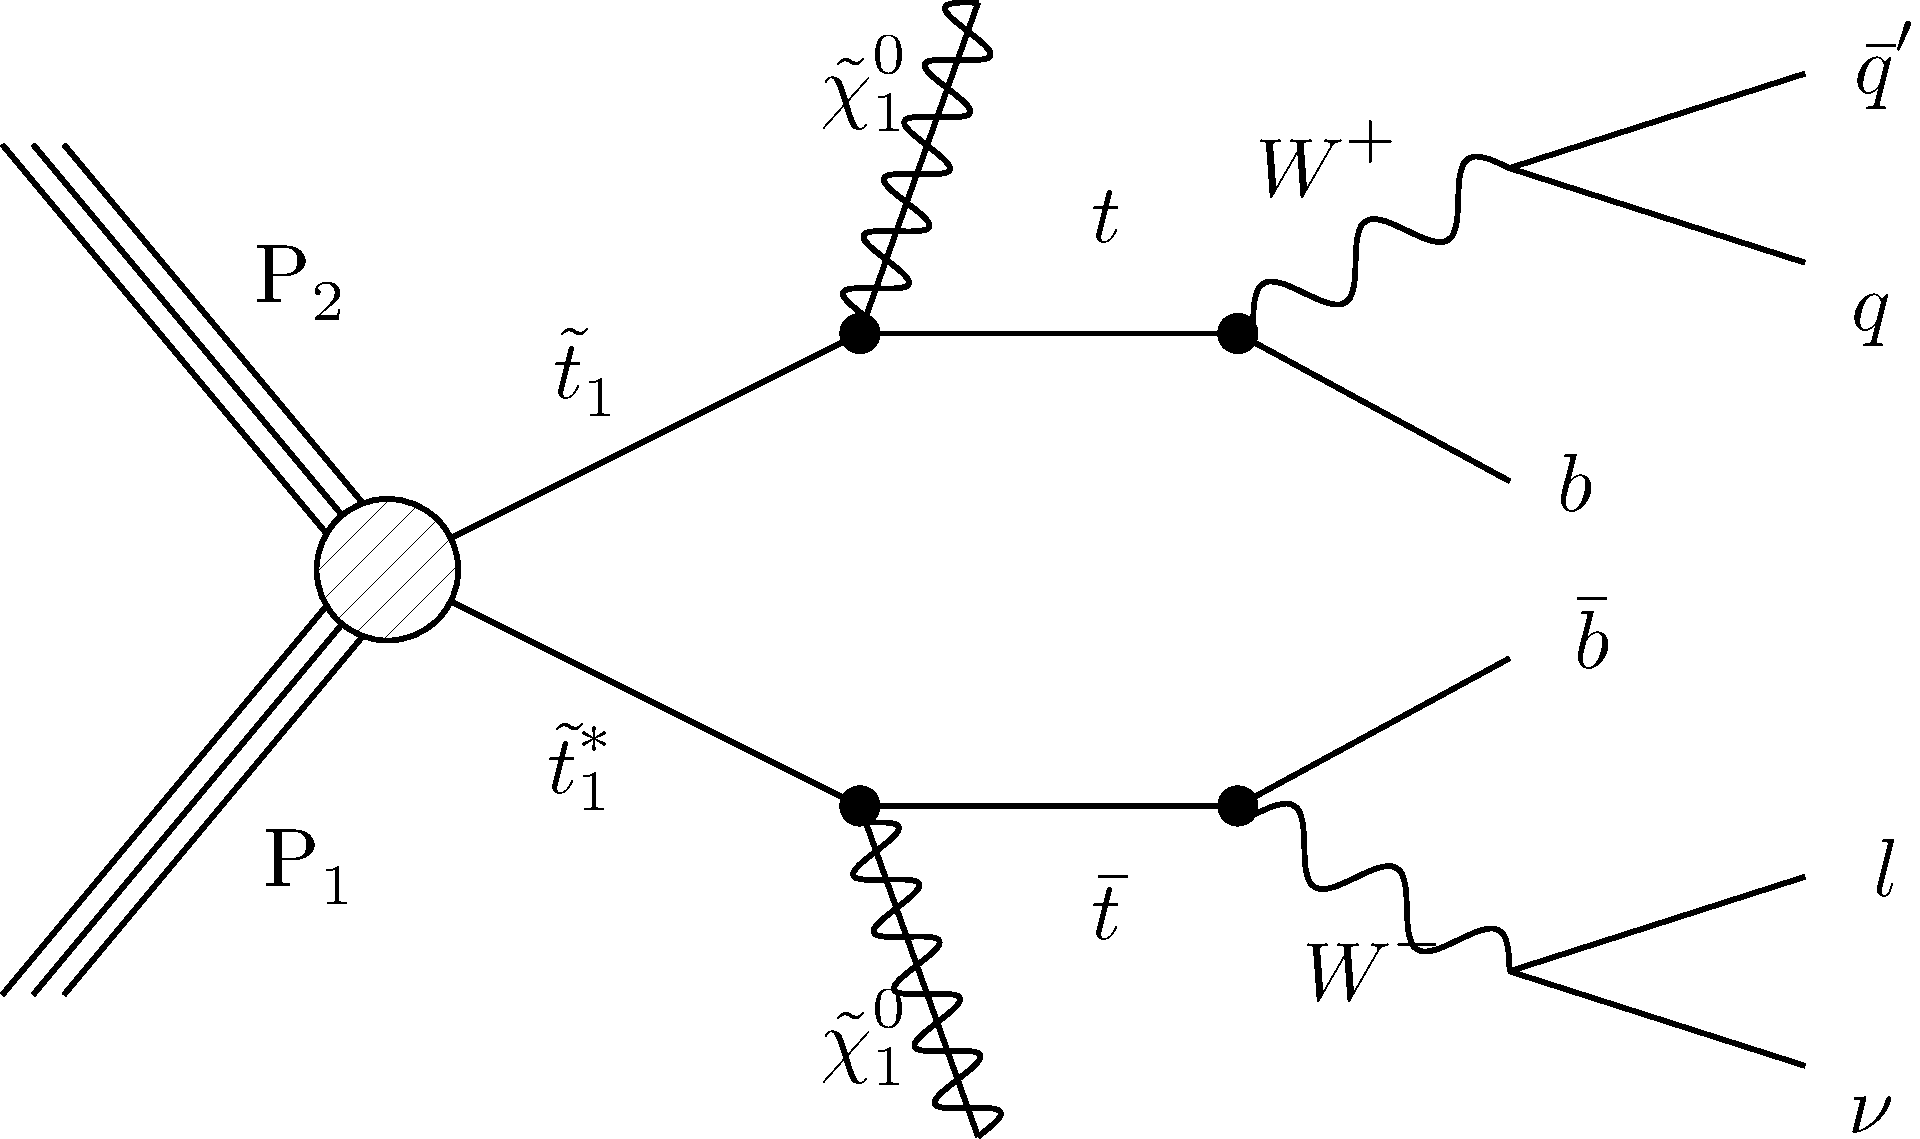
\includegraphics[width=0.45\linewidth]{plots_stop/T2tt1l_feyn.pdf}
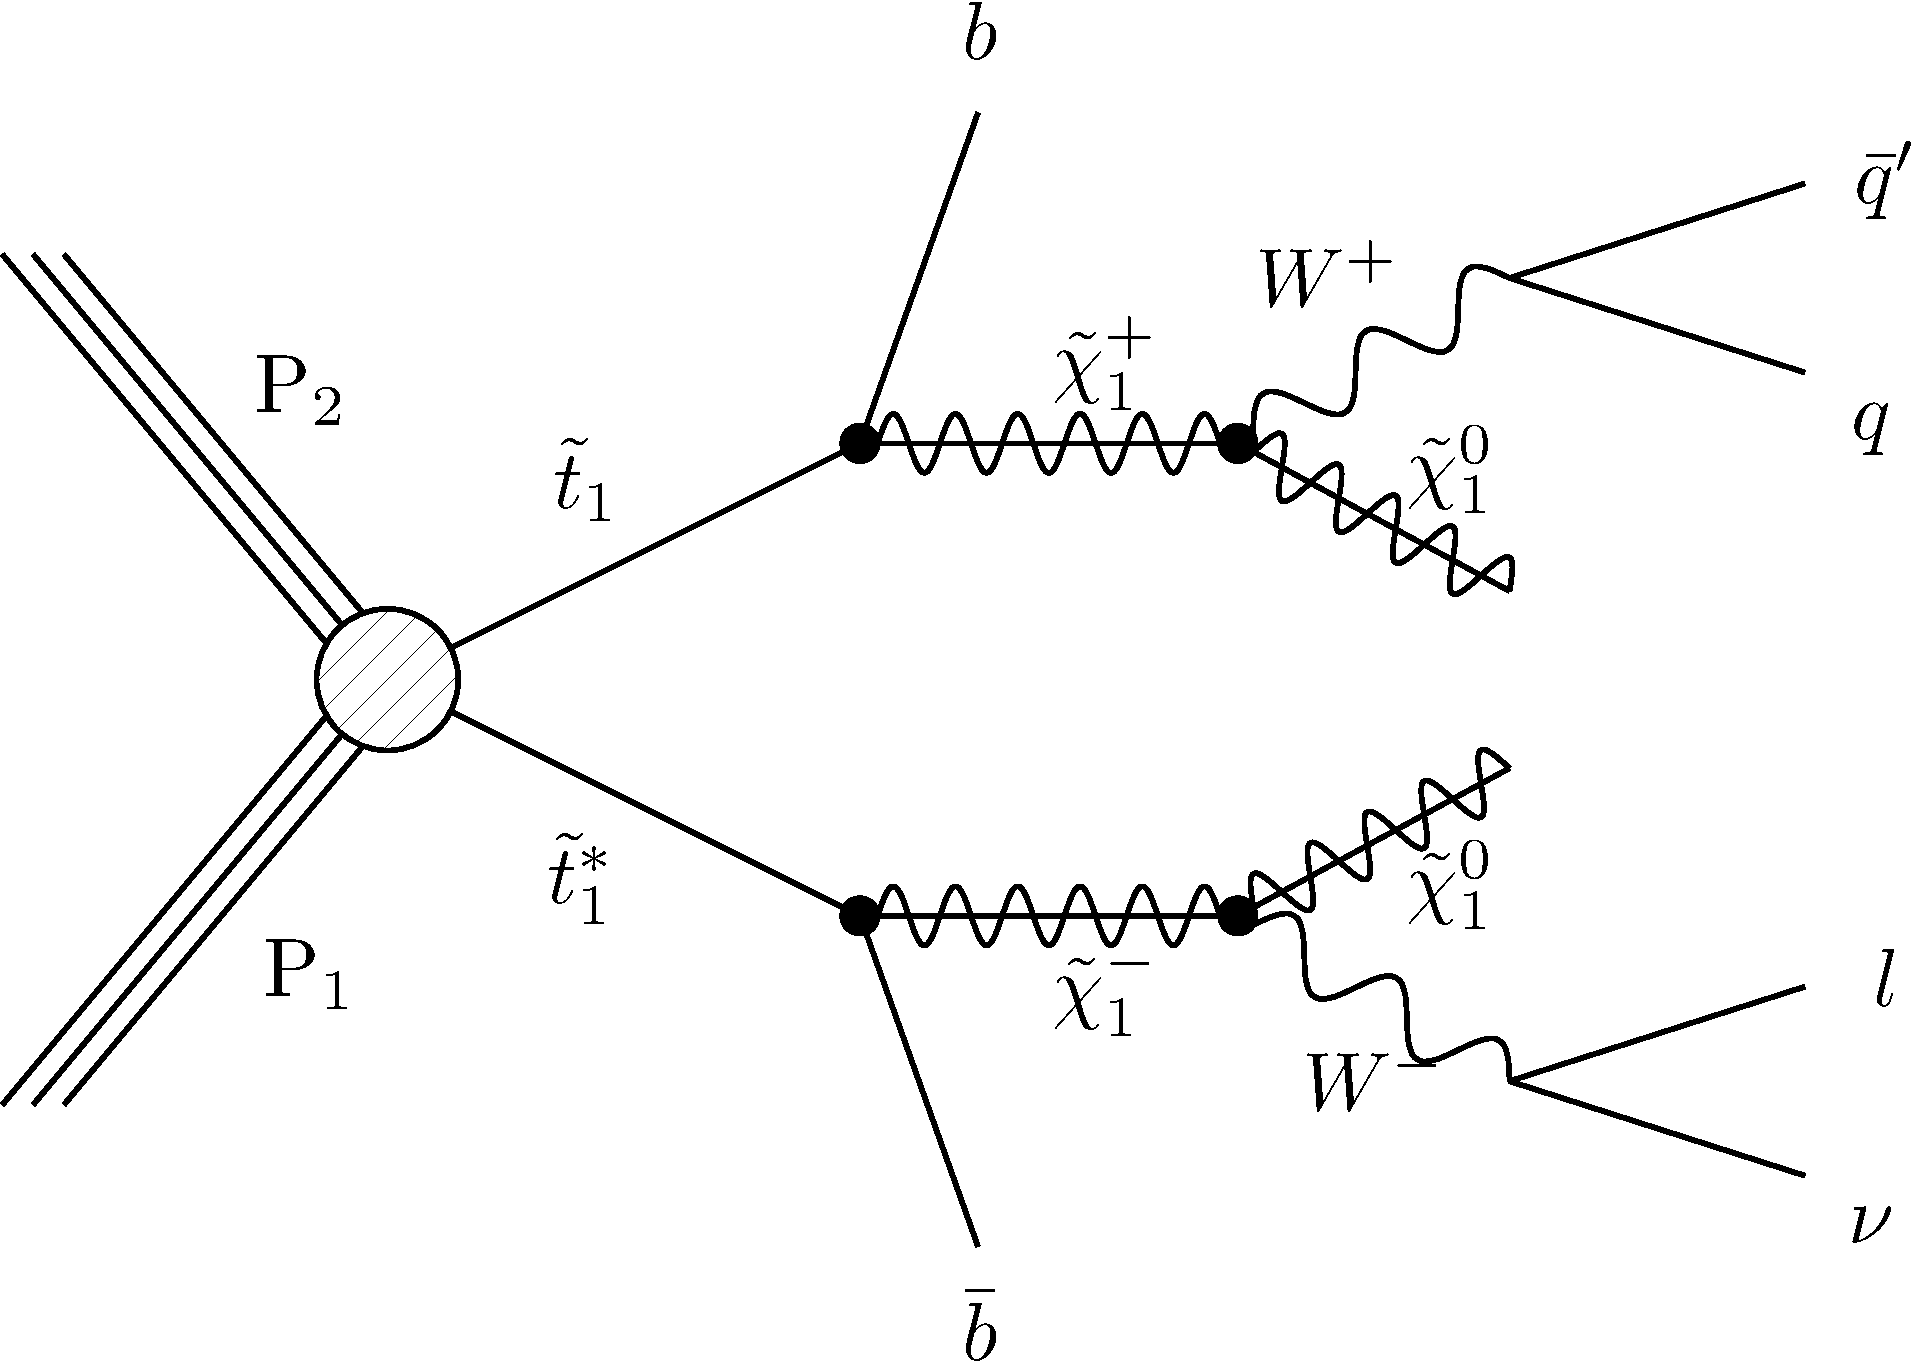
\includegraphics[width=0.45\linewidth]{plots_stop/T2bW1l_feyn.pdf}
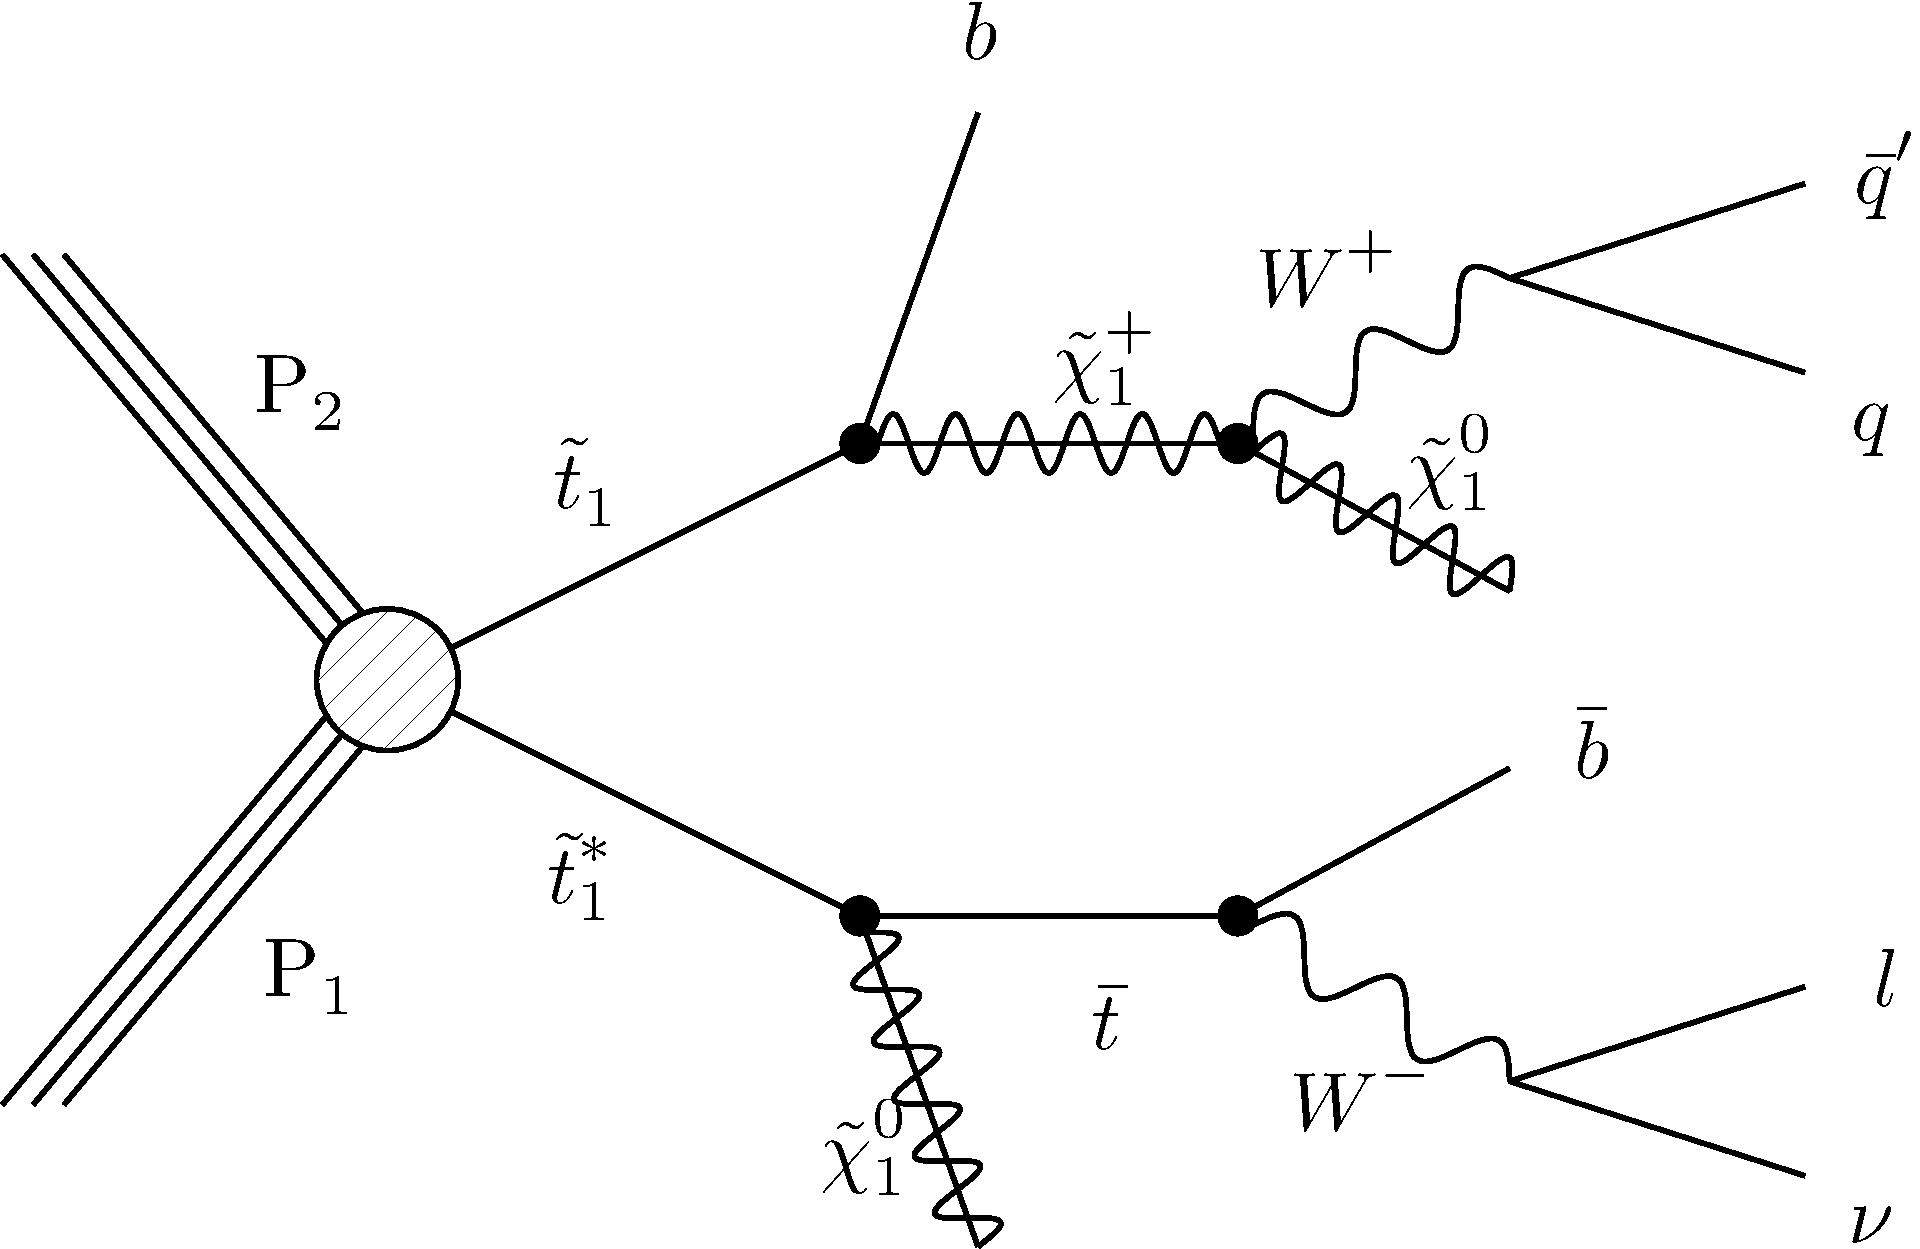
\includegraphics[width=0.45\linewidth]{plots_stop/T2tb1l_feyn.pdf}
\label{sgnProc}
\caption{
  \label{fig:diagram}
        Diagrams for the top squark pair production corresponding to different decay modes shown in Eq.~(1a), (1b), and (1c).}
\end{figure}


\section{Introduction}
\label{sec:intro}
The standard model (SM) has been extremely successful at describing particle physics phenomena for decades. Despite its success, 
the SM suffers from such shortcomings as the hierarchy problem, where fine-tuned cancellations of large quantum corrections to the Higgs 
boson mass are required in order for it to be at the electroweak scale. Therefore, the recent discovery of a Higgs boson completes the 
quest for the SM and yet opens a new horizon in particle physics.

Supersymmetry (SUSY) is an attractive extention to the SM, which is based on a new symmetry between bosons and fermions. It 
predicts the existence of a superpartner for every SM particle, with the same quantum numbers but differing by one half unit of spin. 
In R-parity conserving SUSY models, supersymmetric particles are created in pairs, and the lightest supersymmetric particle (LSP)
is stable.  

The leading divergent contribution to the Higgs boson mass from SM particles arises from the Higgs boson coupling to the top quark. 
SUSY provides a possible way to stabilize it through the addition of contributions from a scalar top quark. Furthermore, it offers a 
number of other attractive features, such as unification of the gauge couplings and dark matter particle candidate (via the stable LSP). 
The relatively low Higgs boson mass of about 125 \GeV implies that light scalar top quark with a mass 
in the hundreds of GeV range is preferred in SUSY. In light of this, searches for strong production of top squark pairs have gained strong 
prominence. 

In this note we present the result of a search for top squark pair production in events with single isolated charged lepton (electron or muon),
jets and significant transverse momentum imbalance. The search was performed on a dataset corresponding to an integrated luminosity of 2.3\fbinv 
of proton-proton (pp) collisions collected at a center-of-mass energy of 13 TeV with the Compact Muon Solenoid (CMS) detctor at the LHC. 
Similar searches were previously reported by the ATLAS and CMS collaborations using datasets of 8 TeV pp collisions and by the CDF 
and D0 collaborations at the Tevatron. No excess above Standard Model (SM) expectations was observed and the results of these searches were 
used to place lower limits on the masses of pair produced top squarks for different decay scenarios. Depending on the decay mode, the results 
probed top squarks with masses in the range of approximately $90-700$\GeV. For small neutralino masses, top squark masses up to 700\GeV were 
excluded at a 95\% confidence level.

With the increase of the LHC collision energy from 8 to 13 TeV, the signal cross-section rises by a factor of 8--12 for top
squarks in mass range $700-1000$\GeV. Therefore, even with smaller 13 TeV dataset, the search has the potential to surpass sensitivity 
of LHC Run 1 to top squark pair production.  

The search presented here focuses on the three processes of interest: 
\begin{subequations}
\begin{align}
\label{sgnProc}
pp\rightarrow\tilde{t_1}\tilde{t_1}^*\rightarrow t^{(*)}\bar{t}^{(*)}\chi^0_1\chi^0_1, \\
pp\rightarrow\tilde{t_1}\tilde{t_1}^*\rightarrow b\bar{b}\chi^+_1\chi^-_1 \rightarrow b\bar{b}W^{+(*)}W^{-(*)} \chi^0_1\chi^0_1,\\
pp\rightarrow\tilde{t_1}\tilde{t_1}^*\rightarrow t^{(*)}\chi^0_1b\chi^+_1, 
\end{align}
\end{subequations}
as illustrated in Figure~\ref{fig:diagram} with one of the $W$ bosons decaying leptonically. 
Here the neutralinos ($\chi^0_1$) and charginos ($\chi^+_1$) are mixtures of the superpartners 
of electroweak gauge bosons and the Higgs boson. The lightest neutralino $\chi^0_1$ is often considered to be the LSP 
which escapes without detection and results in large imbalance in transverse momentum. The main backgrounds in the single lepton 
topology are semi-leptonic decays of \ttbar and \wjets. While the first two processes (1a and 1b) have 
already been searched for during Run-1, the mixed decay mode (1c) is being explored with dedicated search regions for the first time.
Under the hypothesis of almost degenerated $\tilde{t}_{1}$ and $\chi_{1}^{0}$, this process can be observed in a final state with an 
isolated lepton, two bottom quarks and transverse momentum imbalance.

\begin{figure}[!htpb]
\centering
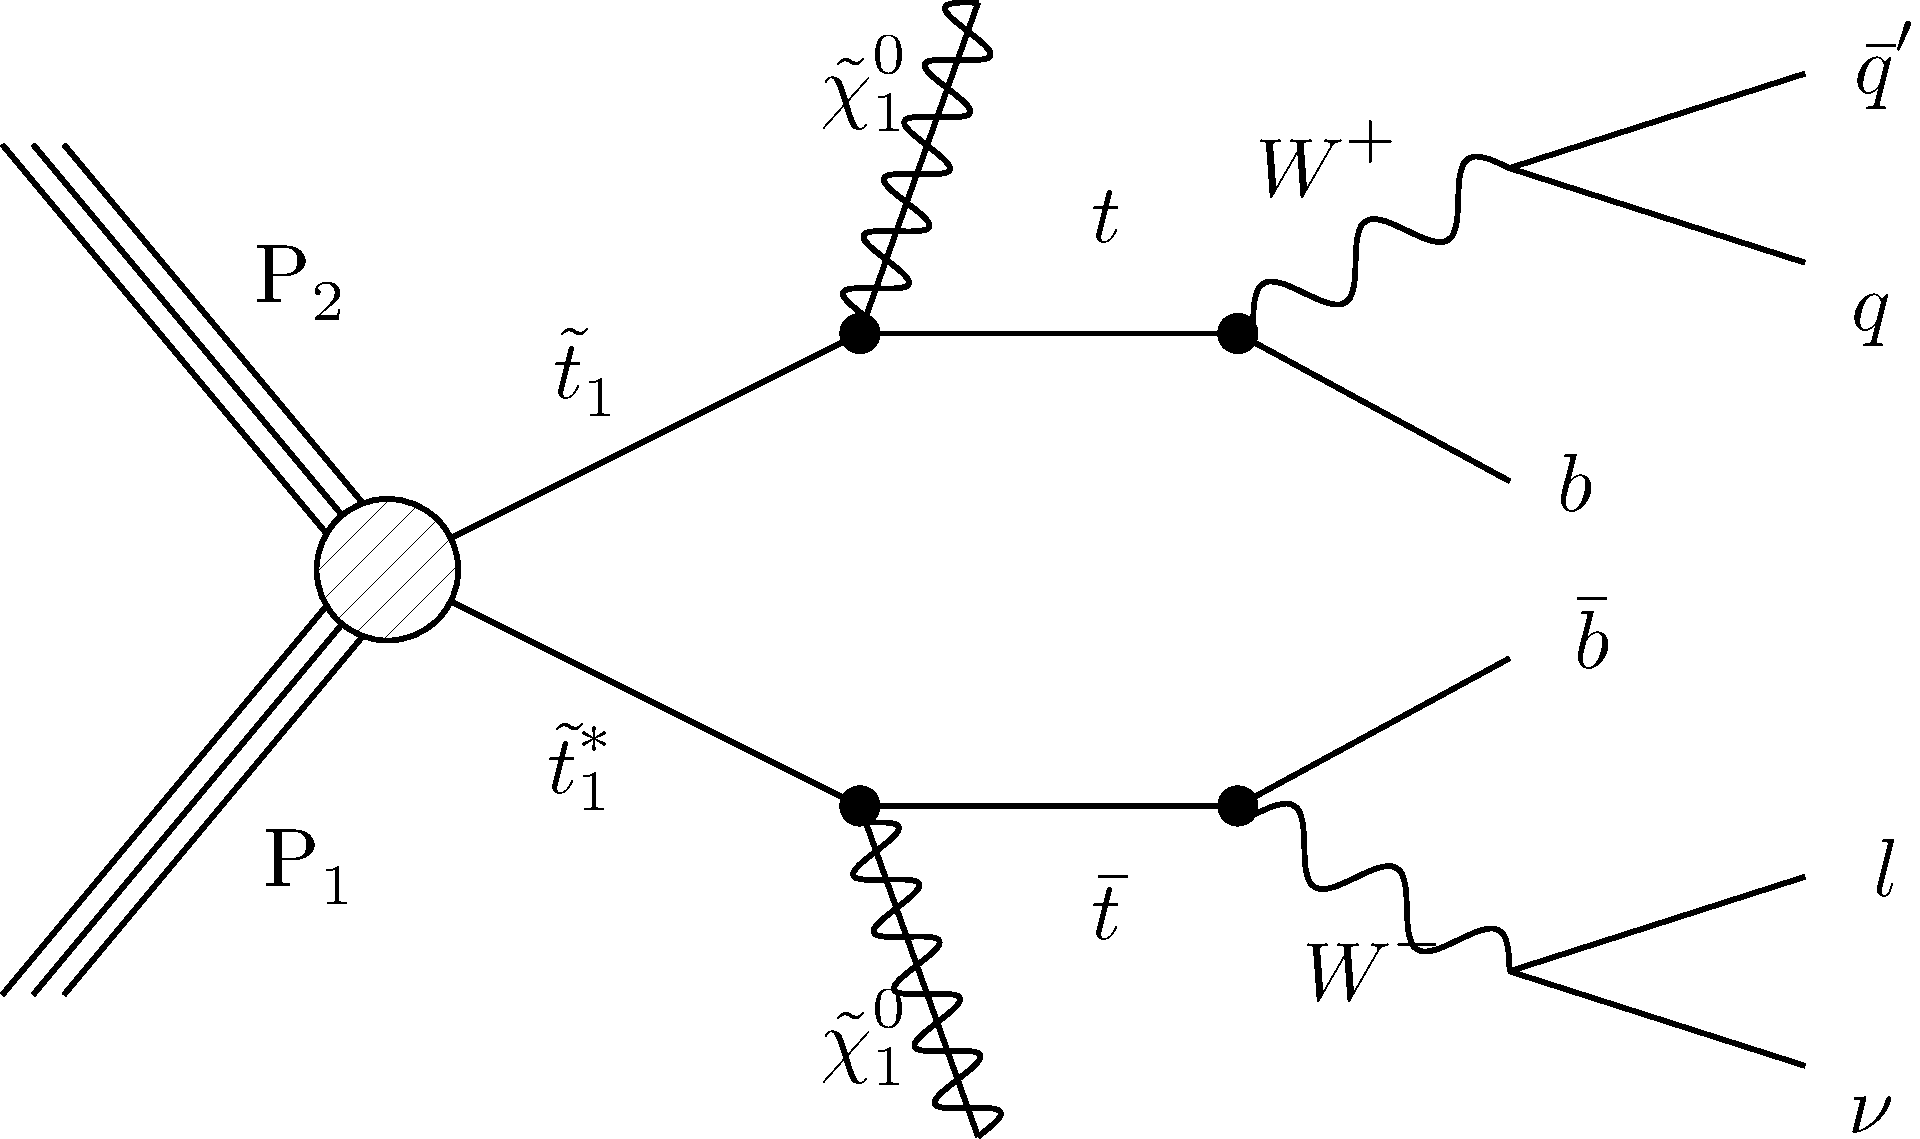
\includegraphics[width=0.45\linewidth]{plots_stop/T2tt1l_feyn.pdf}
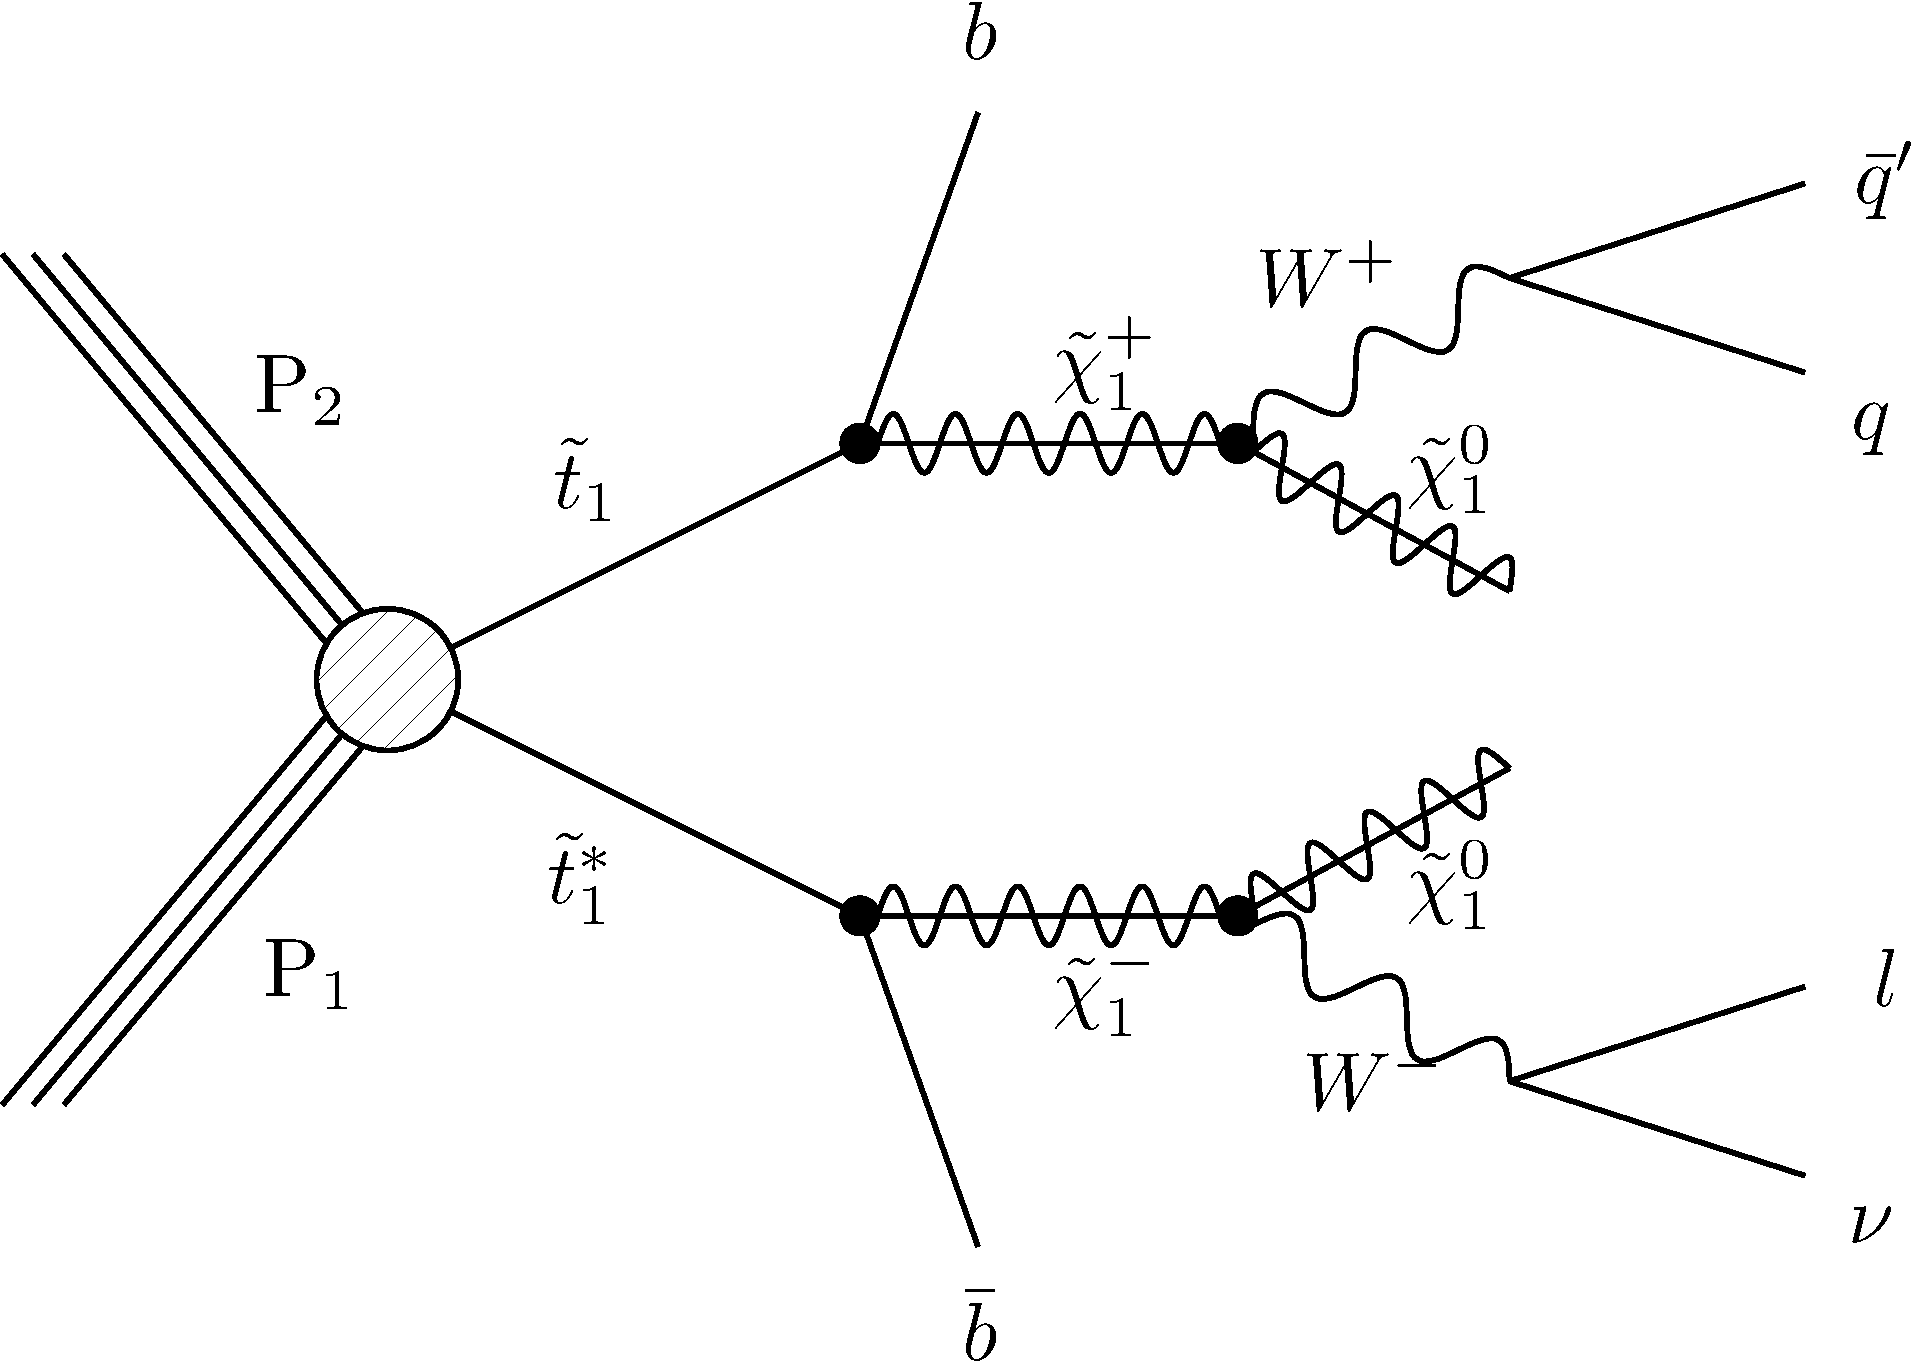
\includegraphics[width=0.45\linewidth]{plots_stop/T2bW1l_feyn.pdf}
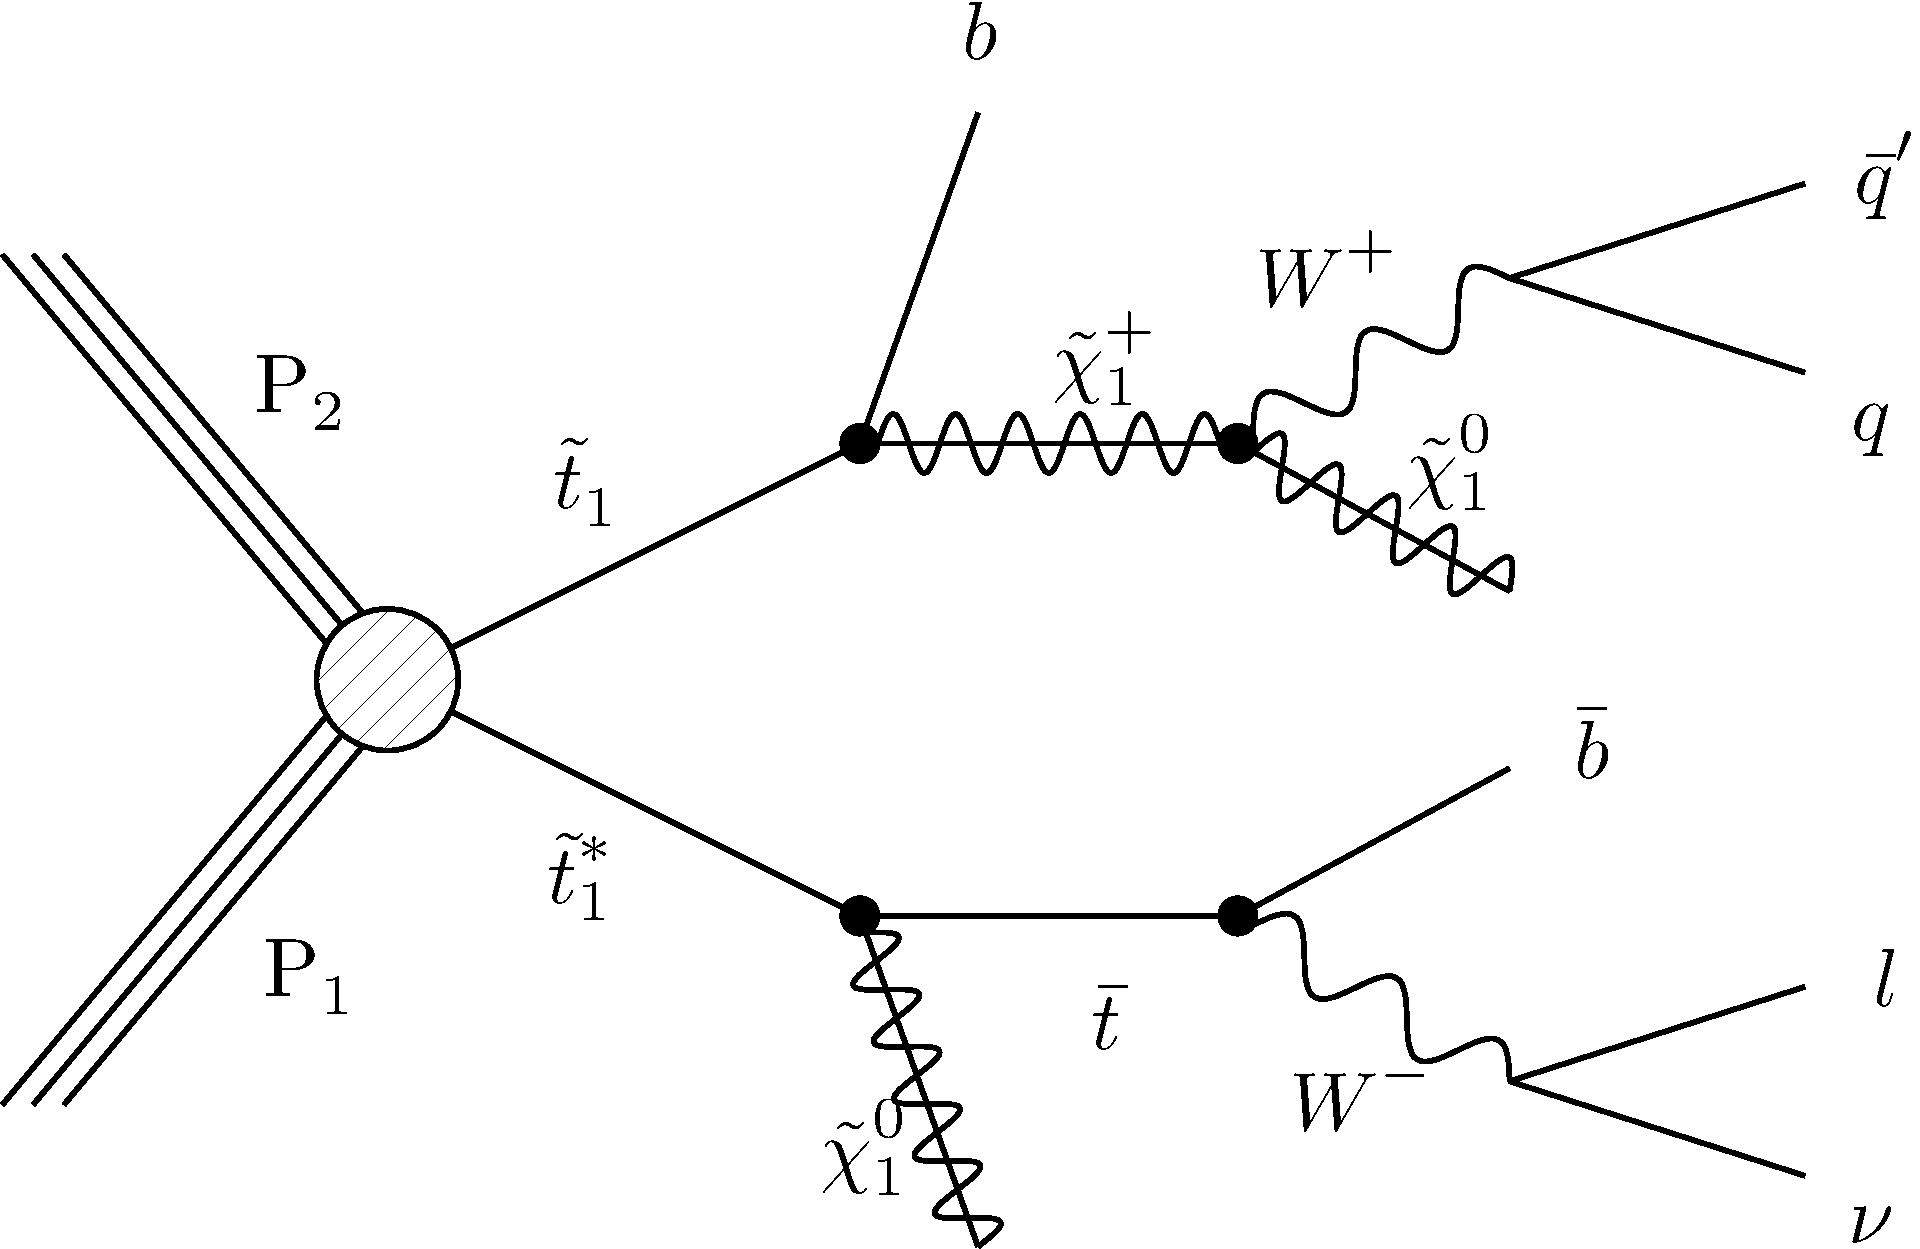
\includegraphics[width=0.45\linewidth]{plots_stop/T2tb1l_feyn.pdf}
\label{sgnProc}
\caption{
  \label{fig:diagram} 
	Diagrams for the top squark pair production corresponding to different decay modes shown in Eq.~(1a), (1b), and (1c).}
\end{figure}

%\section{The CMS detector}

The central feature of the CMS apparatus is a superconducting solenoid of 6\unit{m} internal diameter, 
providing a magnetic field of 3.8\unit{T}. Within the solenoid volume are a silicon pixel and strip tracker, a 
lead tungstate crystal electromagnetic calorimeter, and a brass and scintillator hadron calorimeter, each composed of 
a barrel and two endcap sections. Forward calorimeters extend the pseudorapidity~\cite{JINST} coverage provided by the
 barrel and endcap detectors. Muons are measured in gas-ionization detectors embedded in the steel flux-return yoke outside 
the solenoid. The first level of the CMS trigger system, composed of custom hardware processors, uses information from the 
calorimeters and muon detectors to select the most interesting events in a fixed time interval of less than 4\mus. The high-level
 trigger processor farm further decreases the event rate from around 100\unit{kHz} to less than 1\unit{kHz}, before data storage. 
A more detailed description of the CMS detector, together with a definition of the coordinate system used and the relevant 
kinematic variables, can be found in \reference~\cite{JINST}.

\section{The CMS detector}

The central feature of the CMS apparatus is a superconducting solenoid of 6\unit{m} internal diameter, 
providing a magnetic field of 3.8\unit{T}. Within the solenoid volume are a silicon pixel and strip tracker, a 
lead tungstate crystal electromagnetic calorimeter, and a brass and scintillator hadron calorimeter, each composed of 
a barrel and two endcap sections. Forward calorimeters extend the pseudorapidity~\cite{JINST} coverage provided by the
 barrel and endcap detectors. Muons are measured in gas-ionization detectors embedded in the steel flux-return yoke outside 
the solenoid. The first level of the CMS trigger system, composed of custom hardware processors, uses information from the 
calorimeters and muon detectors to select the most interesting events in a fixed time interval of less than 4\mus. The high-level
 trigger processor farm further decreases the event rate from around 100\unit{kHz} to less than 1\unit{kHz}, before data storage. 
A more detailed description of the CMS detector, together with a definition of the coordinate system used and the relevant 
kinematic variables, can be found in \reference~\cite{JINST}.


%\section{Event samples, reconstruction, and selection}
\subsection{Object definition and event preselection}
\label{sec:presel}
The particle-flow (PF) algorithm~\cite{CMS-PAS-PFT-09-001,CMS-PAS-PFT-10-001} is used to reconstruct and 
identify each individual particle with an optimized combination of information from the various elements of the CMS detector.

The majority of data events are selected using trigger that requires large missing transverse momentum. The missing transverse momentum 
vector \ptvecmiss is defined as the projection on the plane perpendicular to the beams of the negative vector sum of the momenta of all 
reconstructed particles in an event. Its magnitude is referred to as \ETmiss. In the trigger selection, $\ETmiss>170\GeV$ is required. 
Use of this trigger alone introduces a small inefficiency with respect to the offline selection of $\MET > 250\GeV$. To recover the efficiency, 
additional triggers are used. These triggers require presence of at least one lepton (electron or muon) with transverse momentum (\pt) 
requirements of greater than $23\GeV$ for the muon and $20\GeV$ for the electron. The combined trigger efficiency, as measured with a data 
sample of events with large scalar sum of jet transverse momenta ($H_{T}$), varies between XX\% and YY\%(XX\% and YY\%) for events containing 
electrons (muons), each with an uncertainty of about XX\%.

The offline selection requires events to have exactly one lepton with $\pt > 20 \GeV$ and $\abs{\eta} < 2.4$ ($\abs{\eta} < 1.442$) 
for muons (electrons). Electrons in the forward region of the detector are not used due to larger backgrounds. 
Electron candidates are reconstructed starting from a cluster of energy deposits in the
electromagnetic calorimeter. The cluster is then matched to a reconstructed track. The electron selection is based on the shower shape,
track-cluster matching, and consistency between the cluster energy and the track momentum~\cite{Khachatryan:2015hwa}. Muon candidates are 
reconstructed by performing a global fit that requires consistent hit patterns in the tracker and the muon system~\cite{MUOART}.

Leptons are required to be isolated from other activity in the event. A measure of lepton isolation is the scalar \pt\ sum
 ($\pt^\text{sum}$) of all PF particles not associated with the lepton within a cone of radius 
$\Delta R \equiv\sqrt{\smash[b]{(\Delta\eta)^2+(\Delta\phi)^2}}$ dependent on the lepton \pt\:
\begin{align}
\centering
  \Delta R &=\begin{cases}
    0.2, & \pt^{\text{lep}}\leq 50\,\GeV\\
    \frac{10\,\GeV}{\pt^{\text{lep}}}, & 50 \lt\ \pt^{\text{lep}} \le\ 200\,\GeV\\
    0.05, & \pt^{\text{lep}}\geq 200\,\GeV,
  \end{cases}\label{eq:miniIso}
\end{align}
where $\Delta \eta$ ($\Delta \phi$) is the distance in $\eta$ ($\phi$) between the directions of the lepton and the PF particle at 
the primary interaction vertex~\cite{TRK-11-001}. The average contribution of particles from additional \Pp\Pp\ interactions in the 
same or nearby bunch crossings (pileup) is estimated and subtracted from the $\pt^\text{sum}$ quantity. The isolation requirement is
$\pt^\text{sum} <  \min(5\GeV,\, 0.1 \cdot \pt^{\ell})$. Typical lepton identification and isolation efficiencies, measured in
samples of $\ensuremath{\cPZ/\Pgg^\star} \to \ell \ell$ events, are XX\% for electrons and YY\% for muons, with variations at the level of 
a few percent depending on \pt\ and $\eta$.

The PF particles are clustered to form jets using the anti-\kt clustering algorithm~\cite{antikt} with a distance parameter of 0.5, as 
implemented in the {\FASTJET} package~\cite{Cacciari:2011ma}. The contribution to the jet energy from pileup is estimated on an 
event-by-event basis using the jet area method described in \reference~\cite{cacciari-2008-659}, and is subtracted from the overall jet \pt.
Jets from pileup interactions are suppressed using a multivariate discriminant based on the multiplicity of objects clustered in the jet,
the jet shape, and the impact parameters of the charged tracks with respect to the primary interaction vertex. Jets overlapping with 
the selected leptons are not considered in the analysis.

The selected events are required to contain at least two jets with $\pt > 30\GeV$ and $\abs{\eta} < 2.4$. At least one of these jets must 
be consistent with containing the decay of a heavy-flavor hadron, as identified using the medium operating point of the combined secondary 
vertex (CSVv2) bottom quark (b~quark) tagging algorithm~\cite{ref:btag}. We refer to such jets as b-tagged jets. The efficiency of this algorithm 
for b~quark jets in the $\pt$ range 30--400\GeV varies between approximately 60 and 75\% for $\abs{\eta} < 2.4$. The nominal misidentification 
rate for light-quark or gluon jets is approximately 1\%~\cite{ref:btag} for the chosen working point. Corrections are applied to the energy 
measurements of jets to account for non-uniform detector response and  are propagated consistently as a correction to \ptvecmiss. 
The corrected \MET\ magnitude is required to exceed 250\GeV. To reduce effects of instrumentally induced \MET\, we require that the
azimuthal angle between \ptvecmiss and the closest of the two leading $E_{T}$ jets exceeeds 0.8 radians.

To suppress single-lepton backgrounds originating from semi-leptonic \ttbar, 
\wjets, and single top production processes, a requirement on the transverse mass of the lepton-neutrino system
$\MT = \sqrt{2 \pt^{\ell} \MET (1 - cos(\phi))}$ is imposed, where $\phi$ is the angle between the transverse momentum of the lepton and \MET. 
For the background processes containing a single leptonically-decaying $W$ boson, there is a kinematic endpoint $M_{T} < M_{W}$, which can be 
blurred by limited detector resolution and off-shell $W$ mass effects. In this analysis we require $M_{T} > 150\GeV$, which significantly reduces 
single-lepton backgrounds. 

The residual background is dominated by dilepton \ttbar and single top events, where one of the leptons is not reconstructed and the 
presence of the additional neutrino from the second leptonically-decaying $W$ boson allows the event to pass the $M_{T}$ requirement.
In order to reduce this background, we apply loose lepton reconstruction requirements to look for the presence of second electon or muon
with $\pt > 5\GeV$, and reject the event if such a lepton is found. Moreover, events are rejected if, in addition to the selected lepton,
they contain reconstructed hadronic tau decay with $\pt > 20\GeV$ or an isolated track with $\pt > 10\GeV$.


\subsection{Signal Region Definitions}
\label{sec:presel}
Kinematic properties and jet multiplicity in signal events depend on the decay mode of top squarks, as well as on the 
mass splittings between top squark, chargino and neutralino. To achieve better overall sensitivity of the analysis, we optimize
signal region selections separately for signal processes shown in~\ref{sgnProc} and for different mass splitting regions.

As a basis of the search strategy for Eq.~(1a) and (1b) models, we require presence of at least four jets. 
Events are then categorized based on the value of the \MTtW variables~\cite{Bai:2012gs}. The \MTtW variable attempts to reconstruct
the events under the assumption that it has originated in a $\ttbar\rightarrow\ell\ell$ process with one undetected lepton and  
helps to discriminate signal from the dominant dilepton \ttbar background. For large mass differences between the 
top squark and the neutralino, $\Delta$M, the $\MTtW>200\GeV$ requirement significantly reduces the background while preserving good 
signal efficiency. In contrast, for small $\Delta$M such a requirement would result in a loss of large fraction of the signal.
To preserve sensitivity to both high and low $\Delta$M values, we keep all events but divide them in two orthogonal search regions 
with $\MTtW>200\GeV$ and $\MTtW<200\GeV$.

In events with heavy top squarks and small neutralino masses there is a significant probability for the two quarks to merge into a single 
jet due to large boost of hadronically decaying $W$ boson. These events would fail four-jet requirement. To recover acceptance for such topology,
 we define additional search region with 3 jets. Since this region targets signal events with large $\Delta$M values, only events with 
$\MTtW>200\GeV$ are considered.

To increase the sensitivity for the mixed decay scenario model in Eq.~(1c) with nearly degenerate chargino and neutralino, 
a search region with exactly two jets is added. It was found that in these events with low jet multiplicity modified topness 
variable:
\begin{align} \label{eq:modtopness}
t_\mathrm{mod} = \ln(\min S)~\text{ with }~ S(\vec{p}_W, p_{\nu,z}) = \frac{(m_W^2-(p_\nu+p_\ell)^2)^2}{a_W^4} + 
\frac{(m_t^2 - (p_{b}+p_W)^2)^2}{a_t^4}
\end{align}
provides better dilepton \ttbar\ rejection than \MTtW. Here $a_W = 5\GeV$ and $a_t = 15\GeV$ are resolution parameters. 
Events are required to have $t_{mod}>6.4$.

Finally, events in each of the search regions described above are further classified into different signal regions 
based on the value of \MET. Overall, we end up with nine signal regions summarized in Table.~\ref{tab:SR}.
\begin{table}
\begin{center}
\topcaption{\label{tab:SR} Summary of the signal region definitions.}
%\tiny
%\setlength{\tabcolsep}{1pt}
%\vspace{-4pt}
\begin{tabular}{|r|r|r|rrr|}
\hline
$N_{Jets}$ & $M_\mathrm{T2}^W$ [GeV] & $t_\mathrm{mod}$ & \multicolumn{3}{c|}{$E_\mathrm{T}^\mathrm{miss}$ [GeV]} \\
\hline
$\geq4$ & $\leq 200$ & & $250$--$325$ & $>325$ & \\
$\geq4$ & $> 200$ & & $250$--$350$ & $350$--$450$ & $>450$ \\
\hline
$=3$ & $>200$ & & $250$--$350$ & $>350$ & \\
\hline
$=2$ & & $>6.4$ & $250$--$350$ & $>350$ & \\
\hline
\end{tabular}
\end{center}
\end{table}


\subsection{Signal and background simulation}
\label{sec:mc}

Signal samples of top squark pair production are generated with \MADGRAPH V5 Monte Carlo (MC) event 
generator interfaced with Pythia V8.1. Background samples of \ttbar\ and single top events are generated using \POWHEG 
with a top quark mass of $m_\cPqt=172.5$~\GeV, the CTEQ6M parton distribution functions (PDF), 
and the parton showering and fragmentation performed using Pythia V8.1.
Samples of \wjets, $\ttbar+\text{boson}$, diboson ($\PW\PW$, $\PW\cPZ$, and $\cPZ\cPZ$), and triboson,
events are generated with \MADGRAPH V5~\cite{Alwall:2011uj}.

For both signal and background events, pileup interactions are simulated with \PYTHIA\ and superimposed on the hard collisions,
using a pileup multiplicity distribution that reflects the luminosity profile of the analyzed data.
The CMS detector response is simulated using a \GEANTfour-based model~\cite{Geant}.
The simulated events are reconstructed and analyzed with the same software used to process the collision data.

The measured trigger efficiencies are used to weight the simulated events to account for the trigger requirement.
Small differences between the b~tagging efficiencies measured in data and simulation~\cite{ref:btag} are 
corrected using data-to-simulation scale factors to adjust the b~tagging probability in simulated events.
Lepton selection efficiencies (reconstruction, identification, and isolation) are found to be consistent between data and 
simulation.


\section{Event samples, reconstruction, and selection}
\subsection{Object definition and event preselection}
\label{sec:presel}
The particle-flow (PF) algorithm~\cite{CMS-PAS-PFT-09-001,CMS-PAS-PFT-10-001} is used to reconstruct and 
identify each individual particle with an optimized combination of information from the various elements of the CMS detector.

The majority of data events are selected using trigger that requires large missing transverse momentum. The missing transverse momentum 
vector \ptvecmiss is defined as the projection on the plane perpendicular to the beams of the negative vector sum of the momenta of all 
reconstructed particles in an event. Its magnitude is referred to as \ETmiss. In the trigger selection, $\ETmiss>170\GeV$ is required. 
Use of this trigger alone introduces a small inefficiency with respect to the offline selection of $\MET > 250\GeV$. To recover the efficiency, 
additional triggers are used. These triggers require presence of at least one lepton (electron or muon) with transverse momentum (\pt) 
requirements of greater than $23\GeV$ for the muon and $20\GeV$ for the electron. The combined trigger efficiency, as measured with a data 
sample of events with large scalar sum of jet transverse momenta ($H_{T}$), varies between XX\% and YY\%(XX\% and YY\%) for events containing 
electrons (muons), each with an uncertainty of about XX\%.

The offline selection requires events to have exactly one lepton with $\pt > 20 \GeV$ and $\abs{\eta} < 2.4$ ($\abs{\eta} < 1.442$) 
for muons (electrons). Electrons in the forward region of the detector are not used due to larger backgrounds. 
Electron candidates are reconstructed starting from a cluster of energy deposits in the
electromagnetic calorimeter. The cluster is then matched to a reconstructed track. The electron selection is based on the shower shape,
track-cluster matching, and consistency between the cluster energy and the track momentum~\cite{Khachatryan:2015hwa}. Muon candidates are 
reconstructed by performing a global fit that requires consistent hit patterns in the tracker and the muon system~\cite{MUOART}.

Leptons are required to be isolated from other activity in the event. A measure of lepton isolation is the scalar \pt\ sum
 ($\pt^\text{sum}$) of all PF particles not associated with the lepton within a cone of radius 
$\Delta R \equiv\sqrt{\smash[b]{(\Delta\eta)^2+(\Delta\phi)^2}}$ dependent on the lepton \pt\:
\begin{align}
\centering
  \Delta R &=\begin{cases}
    0.2, & \pt^{\text{lep}}\leq 50\,\GeV\\
    \frac{10\,\GeV}{\pt^{\text{lep}}}, & 50 \lt\ \pt^{\text{lep}} \le\ 200\,\GeV\\
    0.05, & \pt^{\text{lep}}\geq 200\,\GeV,
  \end{cases}\label{eq:miniIso}
\end{align}
where $\Delta \eta$ ($\Delta \phi$) is the distance in $\eta$ ($\phi$) between the directions of the lepton and the PF particle at 
the primary interaction vertex~\cite{TRK-11-001}. The average contribution of particles from additional \Pp\Pp\ interactions in the 
same or nearby bunch crossings (pileup) is estimated and subtracted from the $\pt^\text{sum}$ quantity. The isolation requirement is
$\pt^\text{sum} <  \min(5\GeV,\, 0.1 \cdot \pt^{\ell})$. Typical lepton identification and isolation efficiencies, measured in
samples of $\ensuremath{\cPZ/\Pgg^\star} \to \ell \ell$ events, are XX\% for electrons and YY\% for muons, with variations at the level of 
a few percent depending on \pt\ and $\eta$.

The PF particles are clustered to form jets using the anti-\kt clustering algorithm~\cite{antikt} with a distance parameter of 0.5, as 
implemented in the {\FASTJET} package~\cite{Cacciari:2011ma}. The contribution to the jet energy from pileup is estimated on an 
event-by-event basis using the jet area method described in \reference~\cite{cacciari-2008-659}, and is subtracted from the overall jet \pt.
Jets from pileup interactions are suppressed using a multivariate discriminant based on the multiplicity of objects clustered in the jet,
the jet shape, and the impact parameters of the charged tracks with respect to the primary interaction vertex. Jets overlapping with 
the selected leptons are not considered in the analysis.

The selected events are required to contain at least two jets with $\pt > 30\GeV$ and $\abs{\eta} < 2.4$. At least one of these jets must 
be consistent with containing the decay of a heavy-flavor hadron, as identified using the medium operating point of the combined secondary 
vertex (CSVv2) bottom quark (b~quark) tagging algorithm~\cite{ref:btag}. We refer to such jets as b-tagged jets. The efficiency of this algorithm 
for b~quark jets in the $\pt$ range 30--400\GeV varies between approximately 60 and 75\% for $\abs{\eta} < 2.4$. The nominal misidentification 
rate for light-quark or gluon jets is approximately 1\%~\cite{ref:btag} for the chosen working point. Corrections are applied to the energy 
measurements of jets to account for non-uniform detector response and  are propagated consistently as a correction to \ptvecmiss. 
The corrected \MET\ magnitude is required to exceed 250\GeV. To reduce effects of instrumentally induced \MET\, we require that the
azimuthal angle between \ptvecmiss and the closest of the two leading $E_{T}$ jets exceeeds 0.8 radians.

To suppress single-lepton backgrounds originating from semi-leptonic \ttbar, 
\wjets, and single top production processes, a requirement on the transverse mass of the lepton-neutrino system
$\MT = \sqrt{2 \pt^{\ell} \MET (1 - cos(\phi))}$ is imposed, where $\phi$ is the angle between the transverse momentum of the lepton and \MET. 
For the background processes containing a single leptonically-decaying $W$ boson, there is a kinematic endpoint $M_{T} < M_{W}$, which can be 
blurred by limited detector resolution and off-shell $W$ mass effects. In this analysis we require $M_{T} > 150\GeV$, which significantly reduces 
single-lepton backgrounds. 

The residual background is dominated by dilepton \ttbar and single top events, where one of the leptons is not reconstructed and the 
presence of the additional neutrino from the second leptonically-decaying $W$ boson allows the event to pass the $M_{T}$ requirement.
In order to reduce this background, we apply loose lepton reconstruction requirements to look for the presence of second electon or muon
with $\pt > 5\GeV$, and reject the event if such a lepton is found. Moreover, events are rejected if, in addition to the selected lepton,
they contain reconstructed hadronic tau decay with $\pt > 20\GeV$ or an isolated track with $\pt > 10\GeV$.


\subsection{Signal Region Definitions}
\label{sec:presel}
Kinematic properties and jet multiplicity in signal events depend on the decay mode of top squarks, as well as on the 
mass splittings between top squark, chargino and neutralino. To achieve better overall sensitivity of the analysis, we optimize
signal region selections separately for signal processes shown in~\ref{sgnProc} and for different mass splitting regions.

As a basis of the search strategy for Eq.~(1a) and (1b) models, we require presence of at least four jets. 
Events are then categorized based on the value of the \MTtW variables~\cite{Bai:2012gs}. The \MTtW variable attempts to reconstruct
the events under the assumption that it has originated in a $\ttbar\rightarrow\ell\ell$ process with one undetected lepton and  
helps to discriminate signal from the dominant dilepton \ttbar background. For large mass differences between the 
top squark and the neutralino, $\Delta$M, the $\MTtW>200\GeV$ requirement significantly reduces the background while preserving good 
signal efficiency. In contrast, for small $\Delta$M such a requirement would result in a loss of large fraction of the signal.
To preserve sensitivity to both high and low $\Delta$M values, we keep all events but divide them in two orthogonal search regions 
with $\MTtW>200\GeV$ and $\MTtW<200\GeV$.

In events with heavy top squarks and small neutralino masses there is a significant probability for the two quarks to merge into a single 
jet due to large boost of hadronically decaying $W$ boson. These events would fail four-jet requirement. To recover acceptance for such topology,
 we define additional search region with 3 jets. Since this region targets signal events with large $\Delta$M values, only events with 
$\MTtW>200\GeV$ are considered.

To increase the sensitivity for the mixed decay scenario model in Eq.~(1c) with nearly degenerate chargino and neutralino, 
a search region with exactly two jets is added. It was found that in these events with low jet multiplicity modified topness 
variable:
\begin{align} \label{eq:modtopness}
t_\mathrm{mod} = \ln(\min S)~\text{ with }~ S(\vec{p}_W, p_{\nu,z}) = \frac{(m_W^2-(p_\nu+p_\ell)^2)^2}{a_W^4} + 
\frac{(m_t^2 - (p_{b}+p_W)^2)^2}{a_t^4}
\end{align}
provides better dilepton \ttbar\ rejection than \MTtW. Here $a_W = 5\GeV$ and $a_t = 15\GeV$ are resolution parameters. 
Events are required to have $t_{mod}>6.4$.

Finally, events in each of the search regions described above are further classified into different signal regions 
based on the value of \MET. Overall, we end up with nine signal regions summarized in Table.~\ref{tab:SR}.
\begin{table}
\begin{center}
\topcaption{\label{tab:SR} Summary of the signal region definitions.}
%\tiny
%\setlength{\tabcolsep}{1pt}
%\vspace{-4pt}
\begin{tabular}{|r|r|r|rrr|}
\hline
$N_{Jets}$ & $M_\mathrm{T2}^W$ [GeV] & $t_\mathrm{mod}$ & \multicolumn{3}{c|}{$E_\mathrm{T}^\mathrm{miss}$ [GeV]} \\
\hline
$\geq4$ & $\leq 200$ & & $250$--$325$ & $>325$ & \\
$\geq4$ & $> 200$ & & $250$--$350$ & $350$--$450$ & $>450$ \\
\hline
$=3$ & $>200$ & & $250$--$350$ & $>350$ & \\
\hline
$=2$ & & $>6.4$ & $250$--$350$ & $>350$ & \\
\hline
\end{tabular}
\end{center}
\end{table}


\subsection{Signal and background simulation}
\label{sec:mc}

Signal samples of top squark pair production are generated with \MADGRAPH V5 Monte Carlo (MC) event 
generator interfaced with Pythia V8.1. Background samples of \ttbar\ and single top events are generated using \POWHEG 
with a top quark mass of $m_\cPqt=172.5$~\GeV, the CTEQ6M parton distribution functions (PDF), 
and the parton showering and fragmentation performed using Pythia V8.1.
Samples of \wjets, $\ttbar+\text{boson}$, diboson ($\PW\PW$, $\PW\cPZ$, and $\cPZ\cPZ$), and triboson,
events are generated with \MADGRAPH V5~\cite{Alwall:2011uj}.

For both signal and background events, pileup interactions are simulated with \PYTHIA\ and superimposed on the hard collisions,
using a pileup multiplicity distribution that reflects the luminosity profile of the analyzed data.
The CMS detector response is simulated using a \GEANTfour-based model~\cite{Geant}.
The simulated events are reconstructed and analyzed with the same software used to process the collision data.

The measured trigger efficiencies are used to weight the simulated events to account for the trigger requirement.
Small differences between the b~tagging efficiencies measured in data and simulation~\cite{ref:btag} are 
corrected using data-to-simulation scale factors to adjust the b~tagging probability in simulated events.
Lepton selection efficiencies (reconstruction, identification, and isolation) are found to be consistent between data and 
simulation.


%\input{background.tex}
\section{Background estimation}
\label{Sec:BkgEst}

As outlined above, the largest background in the search regions originates from the \ttbar production, where both top quarks decay leptonically ($\ttbar\rightarrow 2l$) and one of the leptons is not identified due to limited detector acceptance or inefficiency of identification requirements. A smaller contribution to the lost lepton background comes from single t production in association with a W boson.  The lost lepton background is estimated using a dileptonic control region.  The SM background with one real lepton comes from W decays, either through direct W production or via W bosons from top decays.  The neutrino from the W decay is the dominant source of real \MET.  Our baseline cuts of $\MET>250 GeV$ and $\MT>150 GeV$ suppress this background significantly.    The suppression is smaller for the direct W bosons because the top mass functions as a kinematic constraint on the W mass in ttbar. As a result, the high transverse mass tail in ttbar 1-lepton events is dominated by \MET resolution effects, while for W+jets it is largely driven by physics, i.e. the width of the W.   In the search regions where the contribution from W+jets background is significant, we predict the background by extrapolating from a control region with a b-jet veto.  In the other regions and for the ($\ttbar\rightarrow 1l$) background we will be relying on simulation.  Finally also some SM processes with small cross sections will be part of the background to the search.  The dominant one is \ttbar production in association with a Z boson, where the Z boson decays into two neutrinos.  Smaller contributions come from the other processes where \ttbar is produced in association with a vector boson (ttW, tt$\gamma$), and processes with two or three electroweak vector bosons. Multijet backgrounds are negligible in this search because we require a high-$\pt$ lepton, large \MET, large \MT, at least 1 b-tagged jet and also a large azimuthal angle between the \MET and the highest-$\pt$ jets.

\subsection{Lost lepton background}\label{sec:dilepton}
The lost lepton background is estimated from data in a control region that requires a second lepton, passing the veto requirements, or the presence of an isolated track or tau.  After the simulation is corrected for differences in the lepton and jet reconstruction efficiencies, we can estimate the contribution in the search region by extrapolating from this data control region using a transfer factor taken from the simulation.   To prevent signal contamination in the tails of \MET and to increase the number of events available for the measurement in the control regions, we decided to only bin in low and high \MTtW and use an additional transfer factor for the binning in jet multiplicity and \MET. To make sure this new transfer factor is correct, the modeling of additional jets due to initial- and final-state-radiation and the modeling of the \MET spectrum are validated using dedicated studies.   Figure \ref{fig:dilepton} shows good agreement between data and simulation in the dilepton control region for the \MET and \MTtW distributions.

\begin{figure}[ht]
\centering
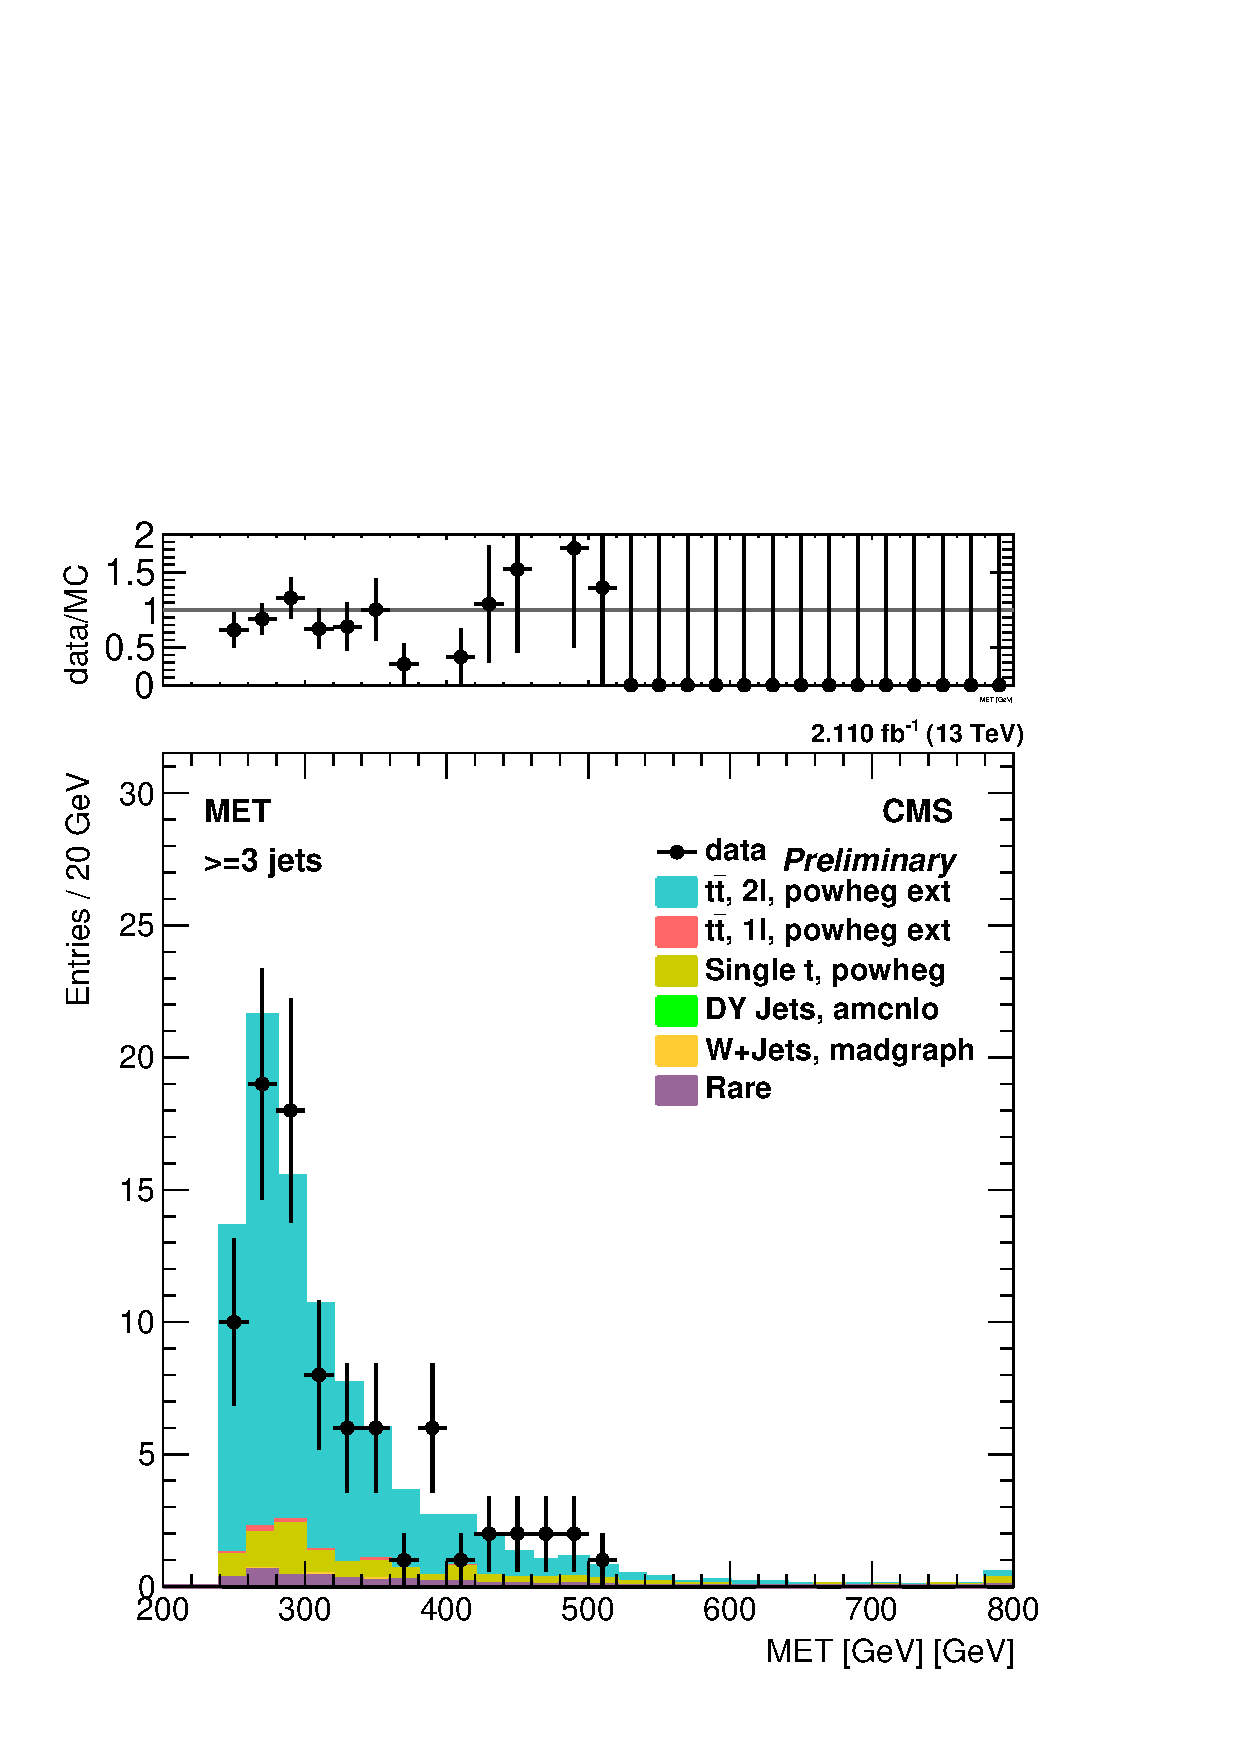
\includegraphics[width=0.45\textwidth]{plots_stop/data_MC_plot__byProductionMode__met__ge3j_ge250met__linScale.pdf}
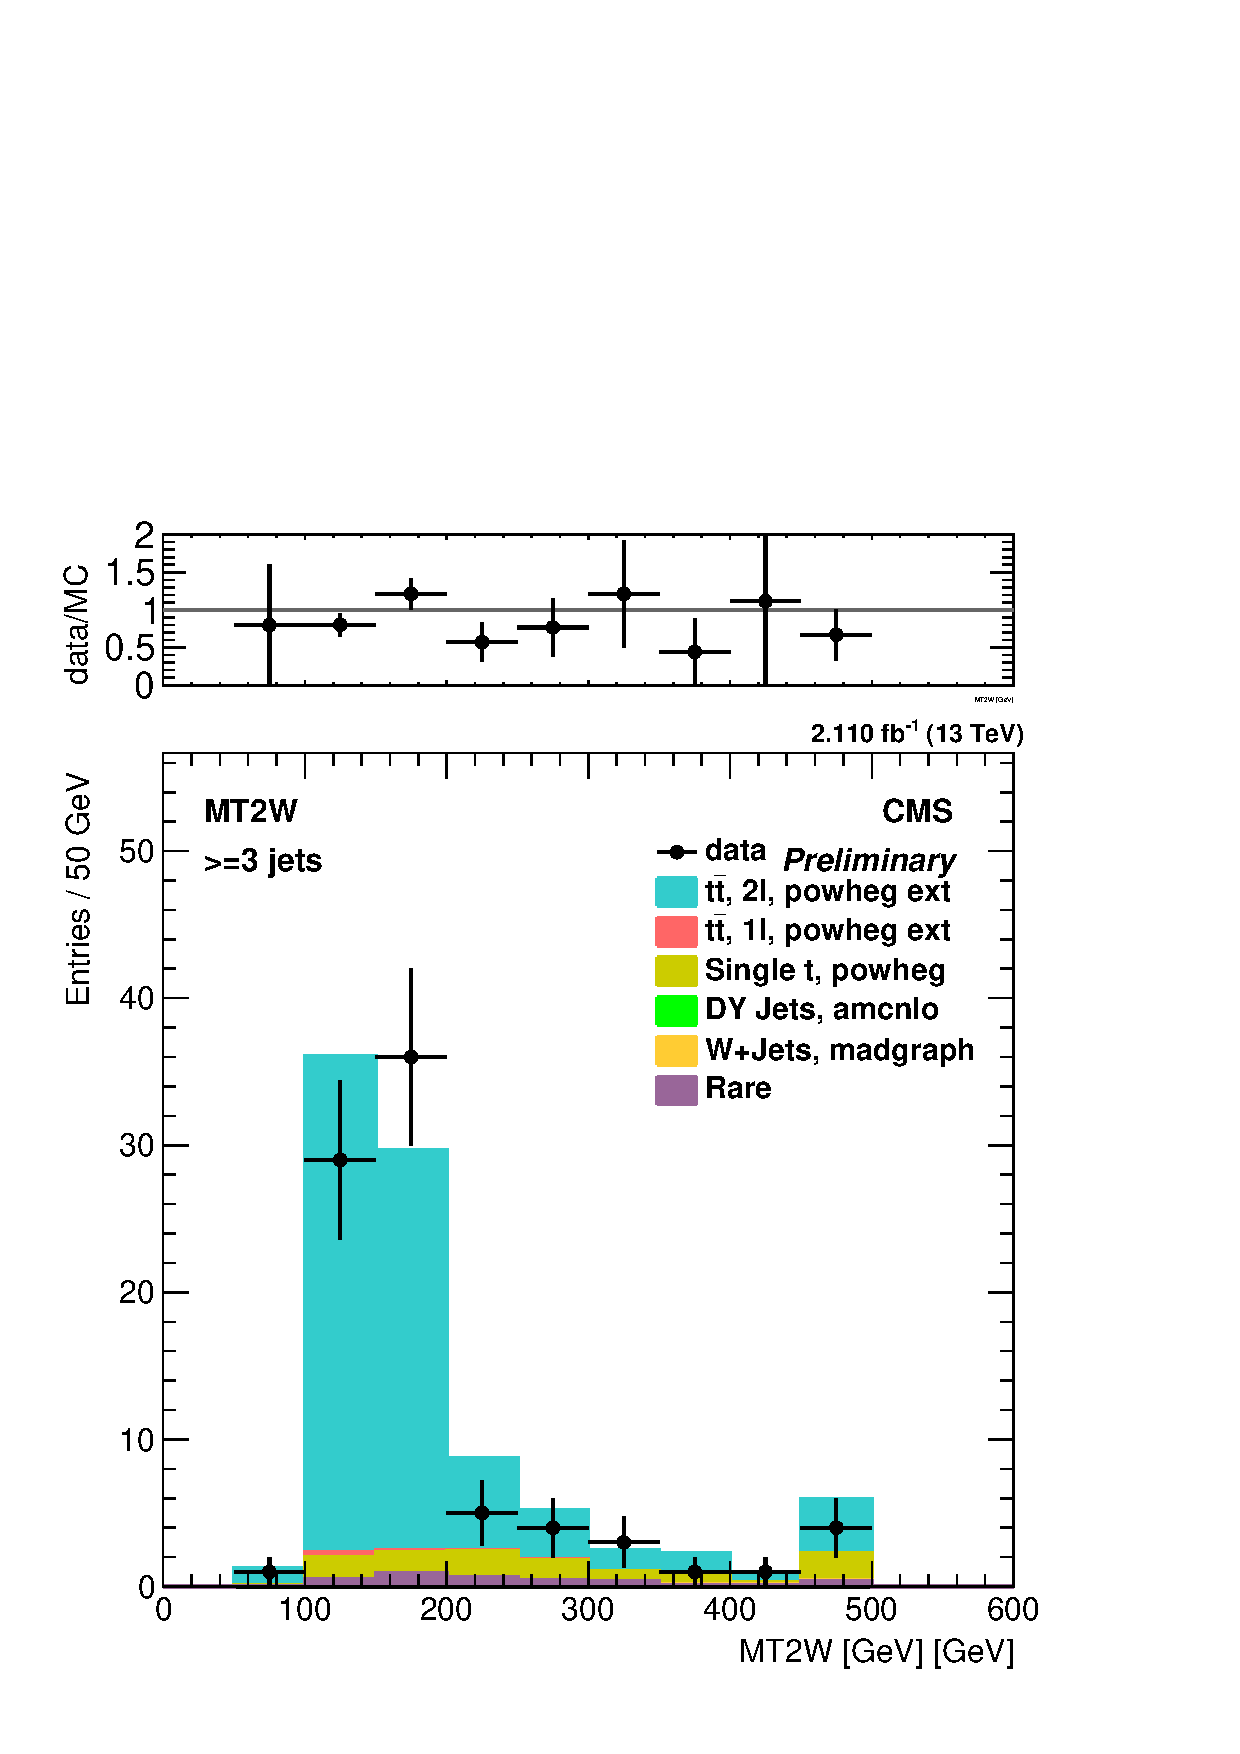
\includegraphics[width=0.45\textwidth]{plots_stop/data_MC_plot__byProductionMode__mt2w__ge3j_ge250met__linScale.pdf}
\caption{\label{fig:dilepton} Good agreement is observed in the dilepton control region for the \MET and \MTtW distributions.}
\end{figure}

$\ttbar\rightarrow 2l$ only contributes to the signal regions with 3 or 4 jets if additional jets from initial-or final-state-radiation are present.  Sometimes also a hadronic tau can be misidentified as an additional jet.  The modeling of the jet multiplicity is checked in a high-purity dedicated $e-\mu$ control region with at least two (b-tagged) jets.  The scale-factors extracted from the comparison between data and simulation are 1.10+/- 0.06 in case we ask for exactly 3 jets and 0.94+/0.06 when we ask for at least 4 jets.  These scale-factors are also checked to be constant with increasing \MET requirements within the statistical uncertainty.

We rely on the simulation to do the correct splitting in \MET bins.  Therefore it is important that we check that the \MET resolution is well-modeled in simulation.  Changing the resolution can lead to a different \MET spectrum and thus bin-to-bin migrations. The uncertainty due to the \MET resolution is estimated by comparing the $\gamma$+jets sample in data and simulation.  The photon \pt spectrum is reweighted to match that from the neutrinos in the background simulation sample.  In case of $\ttbar\rightarrow 2l$ this will be the $\nu\nu$ $\pt$ spectrum.    We then add the transverse momentum of the photon to the MET and then compare the spectrum.   The differences between data and simulation are then applied to the $\ttbar\rightarrow 2l$ simulation and will lead to systematic uncertainties of the order of 2-7\%. Assessing the \MET resolution is also important for the one lepton backgrounds, where we rely on the simulation to determine the transfer factors used for the W+Jets prediction and to assess the small $\ttbar\rightarrow 1l$ contribution.  The systematic uncertainties of the method are described in Sec.\ref{sec:syst}.  The final systematic uncertainty varies between 20 and 47\% for the dilepton backgrounds.

\subsection{One lepton background}\label{sec:onelepton}
After the transverse mass cut the main SM background with one real lepton comes from direct W production as explained earlier.  The best way to get a handle on this background is by looking at a control with no b-tagged jets in the event.  The other cuts for this control region are identical to the baseline selection. For low \MTtW the SM background is completely dominated by the lost lepton background and the one lepton background accounts for less than 10\% of the background everywhere.  A data-driven method is not required and the simulation is used to predict the background.   This is also the case because even the b-vetoed region is dominated by dileptonic \ttbar for low \MTtW.  For high \MTtW we estimate the W+Jets background separately in two bins of exactly 3 jets and at least 4 jets.  
The full \MT distribution for the 0b-tag control region is shown on Fig~\ref{fig:MT}. There is reasonable agreement between data and simulation across the \MT spectrum.   For the large \MT (>150 GeV) region, roughly 35\% of the control regions consists of dileptonic ttbar and invisible Z backgrounds.  Those backgrounds are subtracted to perform the W+Jets estimation, with a 50\% uncertainty assigned to this subtraction.   We then extrapolate the W+Jets yield from the sideband to the signal regions by using a transfer factor from simulation to perform the b-tag and \MET extrapolation.  B-tagging scale factors are applied and also the \MET resolution effects are studied with the study described in Sec.\ref{sec:dilepton}.  After assessing all sources of systematic uncertainties as described in Sec.\ref{sec:syst} , the total uncertainty on the W+Jet estimate varies  between 50 and 70%.

\begin{figure}[h]
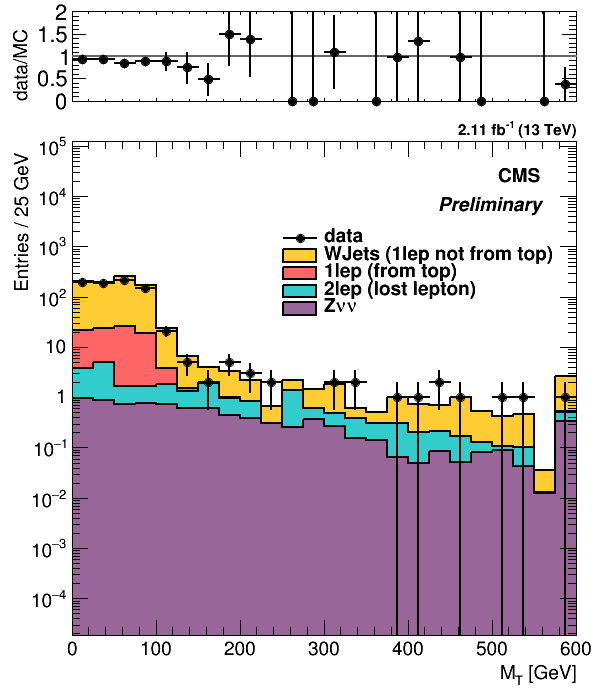
\includegraphics[width=0.44\textwidth]{plots_stop/MTDist_3jets.png}
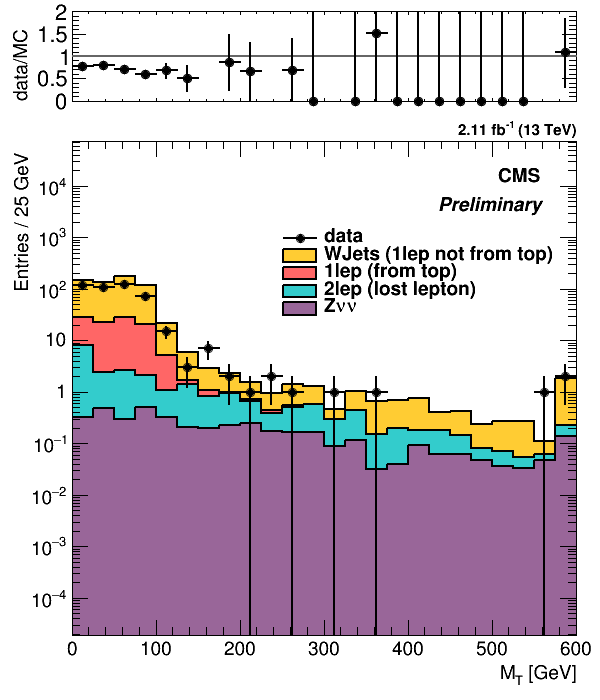
\includegraphics[width=0.44\textwidth]{plots_stop/MTDist_4jets.png}
\caption{\label{fig:MT} Distribution of \MT distribution for 3 jets (left) and $\ge$ 4 jets (right) in the b-vetoed control region with \MET $\ge$ 250\GeV. Good agreement between data and simulation is seen for the full distribution.}
\end{figure}

The $\ttbar\rightarrow 1l$ background is always negligible compared to the other backgrounds.  Therefore we rely on simulation to estimate the background.  The main uncertainty on this estimate is the \MET resolution since the resolution effects could enhance the \MT tail.  The \MET resolution study shows that the resolution could be mismodeled by up to 10\%.  We vary the resolution conservatively by 20\% and take the largest discrepancy in a single \MET bin (100\%)  as the systematic uncertainty on the \ttbar estimate.  
\subsection{Rare Standard Model backgrounds}
The analysis also suffers from rare SM backgrounds, like ttW, ttZ and VV.  It turns out that around 80\% of this background is due to ttZ with $Z\rightarrow\nu\nu$ and this ratio increases with an increasing \MET cut.  Possible control regions, e.g. trileptons, have too few events in the current dataset so we estimate these backgrounds for simulation.  We assess all the theoretical and experimental uncertainties as described in Sec.\ref{sec:syst} and end up with a systematic uncertainty of 15-26\% depending on the exact search region.

%\section{Systematic uncertainties}	
\label{sec:syst}

Most of the sources of systematic uncertainties affect the prediction of both the signal and the background estimates.  They are evaluated separately for the different signal models
and for each hypothesis for the SUSY particle masses. The theoretical uncertainties on the simulation will affect the signal acceptance, the transfer factors used for the one-lepton and dilepton backgrounds and also the estimates of the rare SM backgrounds.  First of all, the effects of missing higher-order corrections to the simulation are assessed.  We estimate these corrections by varying the renormalization and factorization scale up and down by 50\% in our NLO MC samples.  We also estimate the uncertainties of the NNPDF parton distribution functions and the uncertainty on the strong coupling constant.

The experimental uncertainties affect the acceptance for all simulation-based estimates and again the transfer factors for the data-driven estimates.  The uncertainty on the efficiency to estimate b-tags leads to uncertainties on our estimates between 0.5 and 10\%.  $Z\rightarrow ll$ events are used to measure lepton efficiency scale factors and the uncertainties on those varies between 1 and 2\%.  This effect is also propagated to the final signal and background estimates.  For the signal and the rare SM background estimates also the luminosity uncertainty (4.6\%) is propagated.  The uncertainty in the energy scale of  jets gives rise to a 1–15\% systematic uncertainty.  The uncertainty increases with more stringent kinematic requirements.  The modeling of additional pp collisions that overlap with the event of interest leads to an additional uncertainty. The statistical uncertainties on the simulation and data control regions are also taken into account.  

The modeling of initial-state-radiation plays an important role for the signal modeling in case the stop and the LSP mass are very similar.  It is estimated by looking at the initial-state-radiation in Z events.  For the backgrounds it is relevant for the lost lepton background, where we rely on extra radiation for the events to reach the high jet multiplicity bins. This uncertainty is estimated by propagating the uncertainties on the data-simulation ratio in the e$\mu$ control region described in Sec.~\ref{sec:dilepton}.  For the top-related background an additional uncertainty is added due to possible mismodeling of the top transverse momentum distribution.  For the data-driven background estimates also the uncertainty of the \MET resolution, estimated using the $\gamma$+jets method from Sec.~\ref{sec:dilepton}, is important.  For the W+jets background estimate we also assess the effect of changing the W width by its experimental uncertainty.  The modeling of the neutrino $\pt$ spectrum is checked by looking at different \MET bins for events with a transverse mass consistent with the W hypothesis ($60 \GeV<\MT<120 \GeV$). 

Table~\ref{tab:syst} gives a summary of the effect of these different sources on the total uncertainty for our signal and background estimates. The effects that are estimated using the same methods are considered as correlated during our statistical treatment, the other uncertainties and the statistical uncertainties on the different simulation and data control samples are all taken as uncorrelated.

\begin{table}[htb]
\centering
\caption{\label{tab:syst} Summary of the systematic uncertainties for the signal and background estimates with their typical values in individual signal bins. \textcolor{red}{Table needs to be updated.  Also summary for other background estimates needed, asked Indara and John to provide these.} }%, and if the uncertainty can have an effect on the shape.}
\begin{tabular}{lccc}%c}
\hline\hline
Source & \multicolumn{2}{c}{typical size} & correlated \\%& shape effect \\
 & low $\Delta M$ & high $\Delta M$ & \\%& \\
\hline
Signal sample statistics & 10--35\% & 1--10\% & ---  \\%& --- \\
Luminosity & 4.6\% & 4.6\% & $\checkmark$  \\%& --- \\
Trigger & 1\% & 1\% & $\checkmark$  \\%& --- \\
System recoil(``ISR'') & 1--20\% & 1--7\% & $\checkmark$ \\%& $\checkmark$ \\
Jet energy scale & 3--25\% & 1--10\% & $\checkmark$ \\%& $\checkmark$ \\
Renormalization and factorization scale & 1--5\% & 1--3\% & $\checkmark$ \\%& $\checkmark$ \\
b-tagging scale factors & 1--7\% & 1--4\% & $\checkmark$ \\%& $\checkmark$ \\
Lepton efficiency & 1--3\% & 1--3\% & $\checkmark$ \\%& $\checkmark$ \\
Lepton veto efficiency & 3\% & 3\% & --- \\%& --- \\
\hline\hline
\end{tabular}
\end{table}

\section{Systematic uncertainties}	
\label{sec:systematics}

Most of the sources of systematic uncertainties affect the prediction of both the signal and the background estimates.  They are evaluated separately for the different signal models
and for each hypothesis for the SUSY particle masses. The theoretical uncertainties on the simulation will affect the signal acceptance, the transfer factors used for the one-lepton and dilepton backgrounds and also the estimates of the rare SM backgrounds.  First of all, the effects of missing higher-order corrections to the simulation are assessed.  We estimate these corrections by varying the renormalization and factorization scale up and down by 50\% in our NLO MC samples.  We also estimate the uncertainties of the NNPDF parton distribution functions and the uncertainty on the strong coupling constant.
The experimental uncertainties affect the acceptance for all simulation-based estimates and again the transfer factors for the data-driven estimates.  The uncertainty on the efficiency to estimate b-tags leads to uncertainties on our estimates between 0.5 and 10\%.  $Z\rightarrow ll$ events are used to measure lepton efficiency scale factors and the uncertainties on those varies between 1 and 2\%.  This effect is also propagated to the final signal and background estimates.  For the signal and the rare SM background estimates also the luminosity uncertainty (4.6\%) is propagated.  The uncertainty in the energy scale of  jets gives rise to a 1–15% systematic uncertainty.  The uncertainty increases with more stringent kinematic requirements.  The modeling in the simulation of additional pp collisions that overlap with the event of interest leads to an additional uncertainty. The statistical uncertainties on the simulation and data control regions are also taken into account.  

The modeling of initial-state-radiation plays an important role for the signal in case the stop and the LSP mass are very similar.  It is estimated by looking at the initial-state-radiation in Z events.  For the backgrounds it is relevant for the lost lepton background, where we rely on extra radiation for the events to reach the high jet multiplicity bins. This uncertainty is estimate by propagating the uncertainties on the data-simulation ratio in the e$\mu$ control region described in Sec.~\ref{sec:dilepton}.  For the top-related background an additional uncertainty is added due to possible mismodeling of the top transverse momentum distribution.  For the data-driven background estimates also the uncertainty of the \MET resolution, estimated using the $\gamma$+jets method from Sec.~\ref{sec:dilepton}, is important.  For the background estimate for the W+jets background, we also assess the effect of changing the W width by its uncertainty and estimate.  The modeling of the neutrino $\pt$ spectrum is checked by looking at different \MET bins for events with a transverse mass consistent with the W hypothesis ($60 \GeV<\MT<120 \GeV$). 

Table~\ref{tab:syst} gives a summary of the effect of these different sources on the total uncertainty for our signal and background estimates. The effects that are estimated using the same methods are considered as correlated during our statistical treatment, the other uncertainties and the statistical uncertainties on the different simulation and data control samples are all taken as uncorrelated.

\begin{table}[htb]
\centering
\caption{\label{tab:syst} Summary of the systematic uncertainties for the signal and background estimates with their typical values in individual signal bins. \textcolor{red}{Table needs to be updated.  Also summary for other background estimates needed, asked Indara and John to provide these.} }%, and if the uncertainty can have an effect on the shape.}
\begin{tabular}{lccc}%c}
\hline\hline
Source & \multicolumn{2}{c}{typical size} & correlated \\%& shape effect \\
 & low $\Delta M$ & high $\Delta M$ & \\%& \\
\hline
Signal sample statistics & 10--35\% & 1--10\% & ---  \\%& --- \\
Luminosity & 4.6\% & 4.6\% & $\checkmark$  \\%& --- \\
Trigger & 1\% & 1\% & $\checkmark$  \\%& --- \\
System recoil(``ISR'') & 1--20\% & 1--7\% & $\checkmark$ \\%& $\checkmark$ \\
Jet energy scale & 3--25\% & 1--10\% & $\checkmark$ \\%& $\checkmark$ \\
Renormalization and factorization scale & 1--5\% & 1--3\% & $\checkmark$ \\%& $\checkmark$ \\
b-tagging scale factors & 1--7\% & 1--4\% & $\checkmark$ \\%& $\checkmark$ \\
Lepton efficiency & 1--3\% & 1--3\% & $\checkmark$ \\%& $\checkmark$ \\
Lepton veto efficiency & 3\% & 3\% & --- \\%& --- \\
\hline\hline
\end{tabular}
\end{table}


%\section{Results}

A summary of the background expectations and the corresponding data counts for each signal
region is shown in Table \ref{tab:results} and shown in Fig/\ref{fig:results}.  The observed and predicted yields agree in all signal regions within about XX standard deviations. Therefore, we observe no evidence for top-squark pair production.

\begin{table}[htb]
\begin{center}
\caption{\label{tab:results} Results of the data- and simulation-driven background estimates together with the observed data yields for 2.3\fbinv collected during 2015 pp collisions. The uncertainties are the quadratic sums of statistical and systematic uncertainties.{\color{red} Data still blinded.}}
\begin{tabular}{|r|r@{\,$\pm$\,}lr@{\,$\pm$\,}lr@{\,$\pm$\,}lr@{\,$\pm$\,}l|r@{\,$\pm$\,}l|r|}
\hline
\multirow{2}{*}{\MET [GeV]} &  \multicolumn{2}{c|}{\multirow{2}{*}{Lost Lepton}} & \multicolumn{2}{c|}{$1\ell$ (not}  &  \multicolumn{2}{c|}{\multirow{2}{*}{$\ttbar\to1\ell$}} &  \multicolumn{2}{c|}{\multirow{2}{*}{$\cPZ\to\cPgn\cPagn$}} & \multicolumn{2}{c|}{Total} & \multirow{2}{*}{Data} \\
 & \multicolumn{2}{c|}{~} & \multicolumn{2}{c|}{from top)} & \multicolumn{2}{c|}{~} & \multicolumn{2}{c|}{~} & \multicolumn{2}{c|}{background} &  \\
\hline
 & \multicolumn{11}{l|}{Boosted High $\Delta M$}\\%: $3$ jets, $\MTtW>200\GeV$} \\
\hline
$>350$    & 0.84&0.23 & 0.98&0.62 & 0.05&0.05 & 0.28&0.08 & 2.15&0.67 & 0 \\
\hline
 & \multicolumn{11}{l|}{Low $\Delta M$}\\%: $\geq4$ jets, $\MTtW\leq200\GeV$} \\
\hline
$250-325$ & 19.27&2.76 & 0.55&0.55 & 0.76&0.76 & 0.63&0.12 & 21.21&2.92 & 0 \\
$>325$ & 7.64&1.28 & 0.38&0.38 & 0.34&0.34 & 0.27&0.08 & 8.63&1.38 & 0 \\
\hline
 & \multicolumn{11}{l|}{High $\Delta M$}\\%: $\geq4$ jets, $\MTtW>200\GeV$} \\
\hline
$250-350$ & 3.08&0.82 & 1.05&0.53 & 0.49&0.49 & 0.63&0.15 & 5.25&1.10 & 0 \\
$350-450$ & 0.83&0.23 & 0.82&0.49 & 0.12&0.12 & 0.38&0.10 & 2.15&0.56 & 0 \\
$>450$ & 0.59&0.21 & 0.95&0.67 & 0.07&0.07 & 0.34&0.15 & 1.95&0.72 & 0 \\
\hline
\end{tabular}
\end{center}
\end{table}

\begin{figure}[htb]
\centering
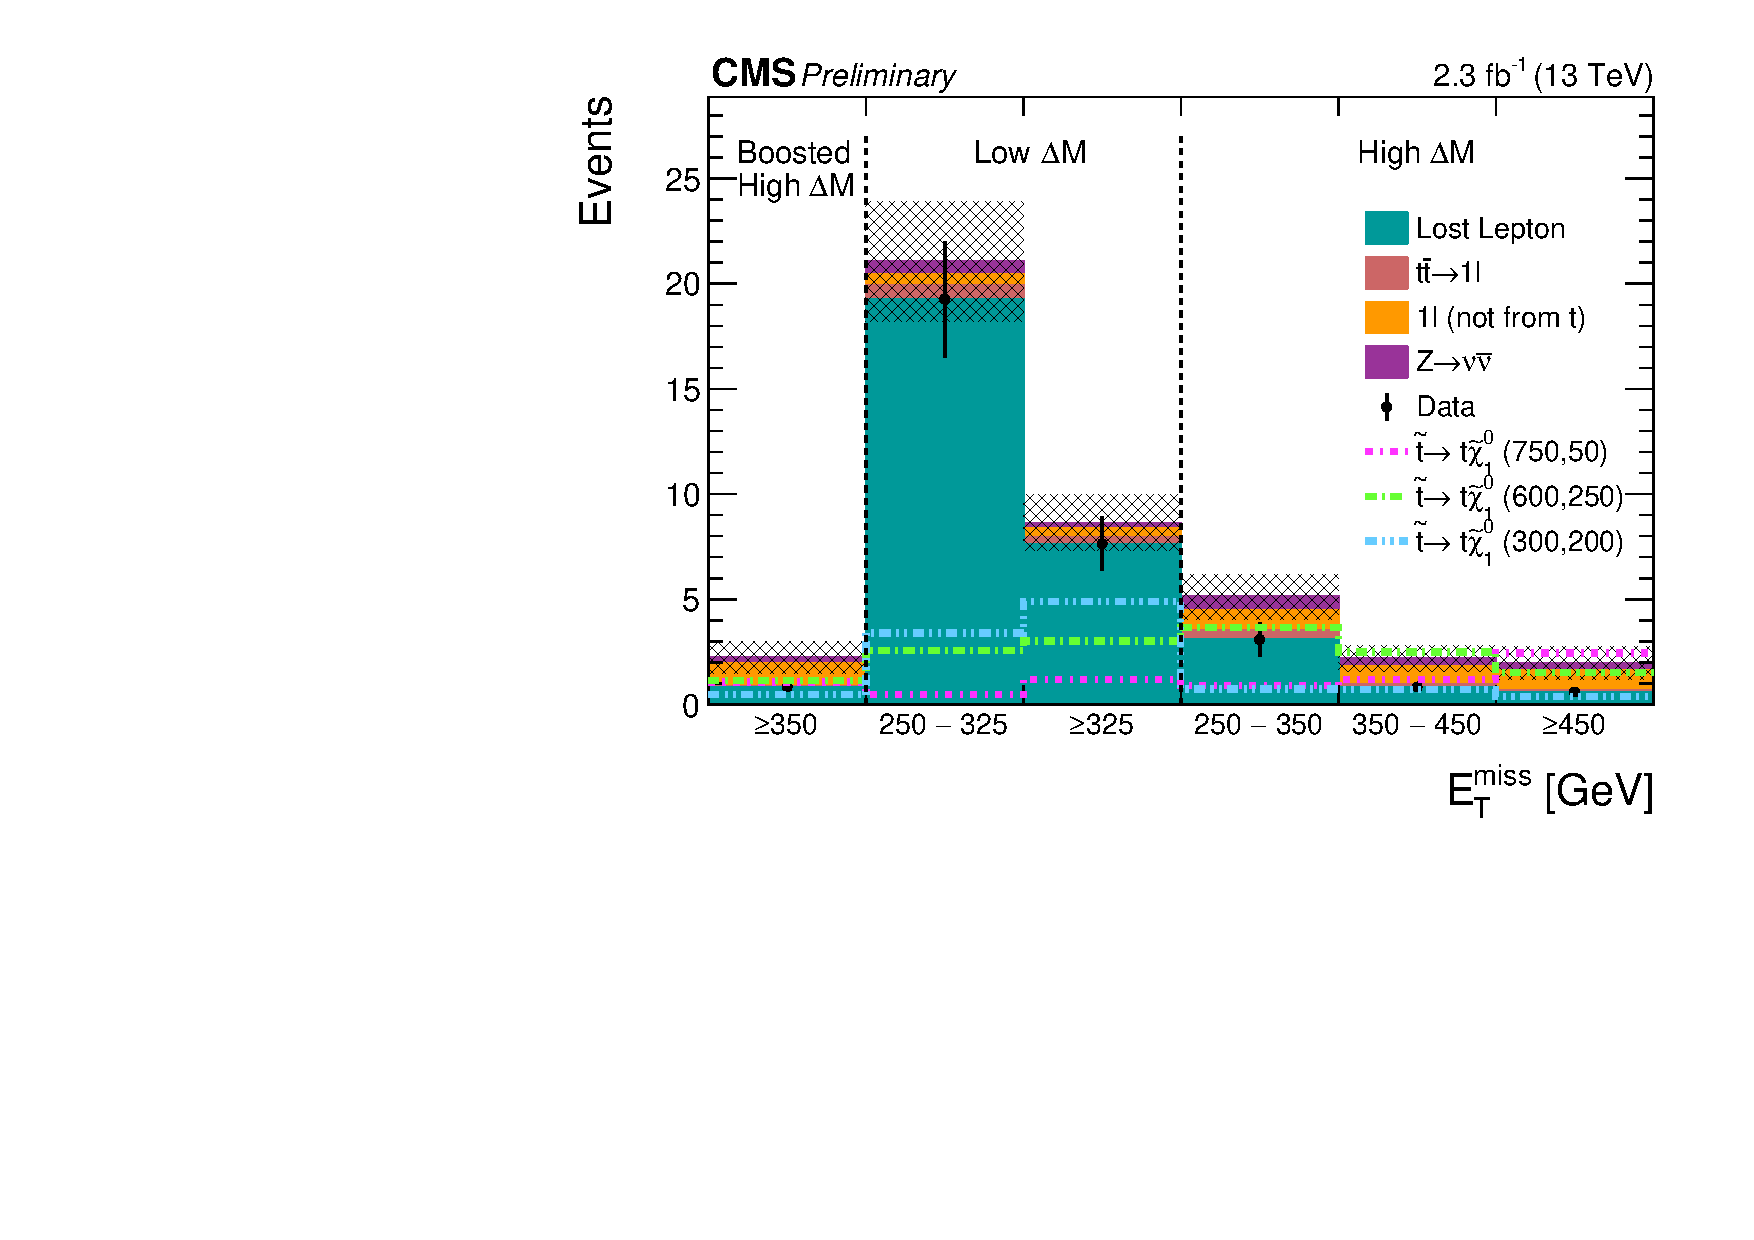
\includegraphics[width=0.90\textwidth]{plots_stop/Results_2p3fbinv.pdf}
\caption{\label{fig:results}Results of the data- and simulation-driven background estimates together with the observed data yields for 2.3\fbinv collected during 2015 pp collisions. The uncertainties, which are the quadratic sums of statistical and systematic uncertainties, are shown as shaded band. Three signal hypotheses are overlaid. {\color{red} Data still blinded, dots here are fake.}}
\end{figure}

The results of the search are interpreted in the context of models of top-squark pair production.  As discussed in Sec.\ref{sec:intro} we consider two different decay modes for the top-squark: directly to a top quark and a LSP or to a bottom quark and a chargino and then the chargino decays to the LSP.  We also consider the option where the chargino is almost mass-degenerate with the LSP.  In that case we can be sensitive to the mixed scenario, where one top decays to a top quark and a LSP and the other one to a bottom quark, a soft and undetected W boson and a LSP.  The systematic uncertainties are discussed in length in Sec.\ref{syst}.  We use all the search bins to calculate 95\% confidence level (CL) upper limits (UL) on the cross sections.  We calculate these upper limits using the LHC style CL$_{S}$ method\cite{Higgscombine}.

Figure~\ref{fig:limits:T2tt} shows the 95\% CL exclusion limits for $\Pp\Pp\to\stone\stone^*\to \PQt^{(*)}\PAQt^{(*)}\PSGczDo\PSGczDo$, together with the upper limit at 95\% CL on the excluded signal cross section.
\begin{figure}[htb]
\centering
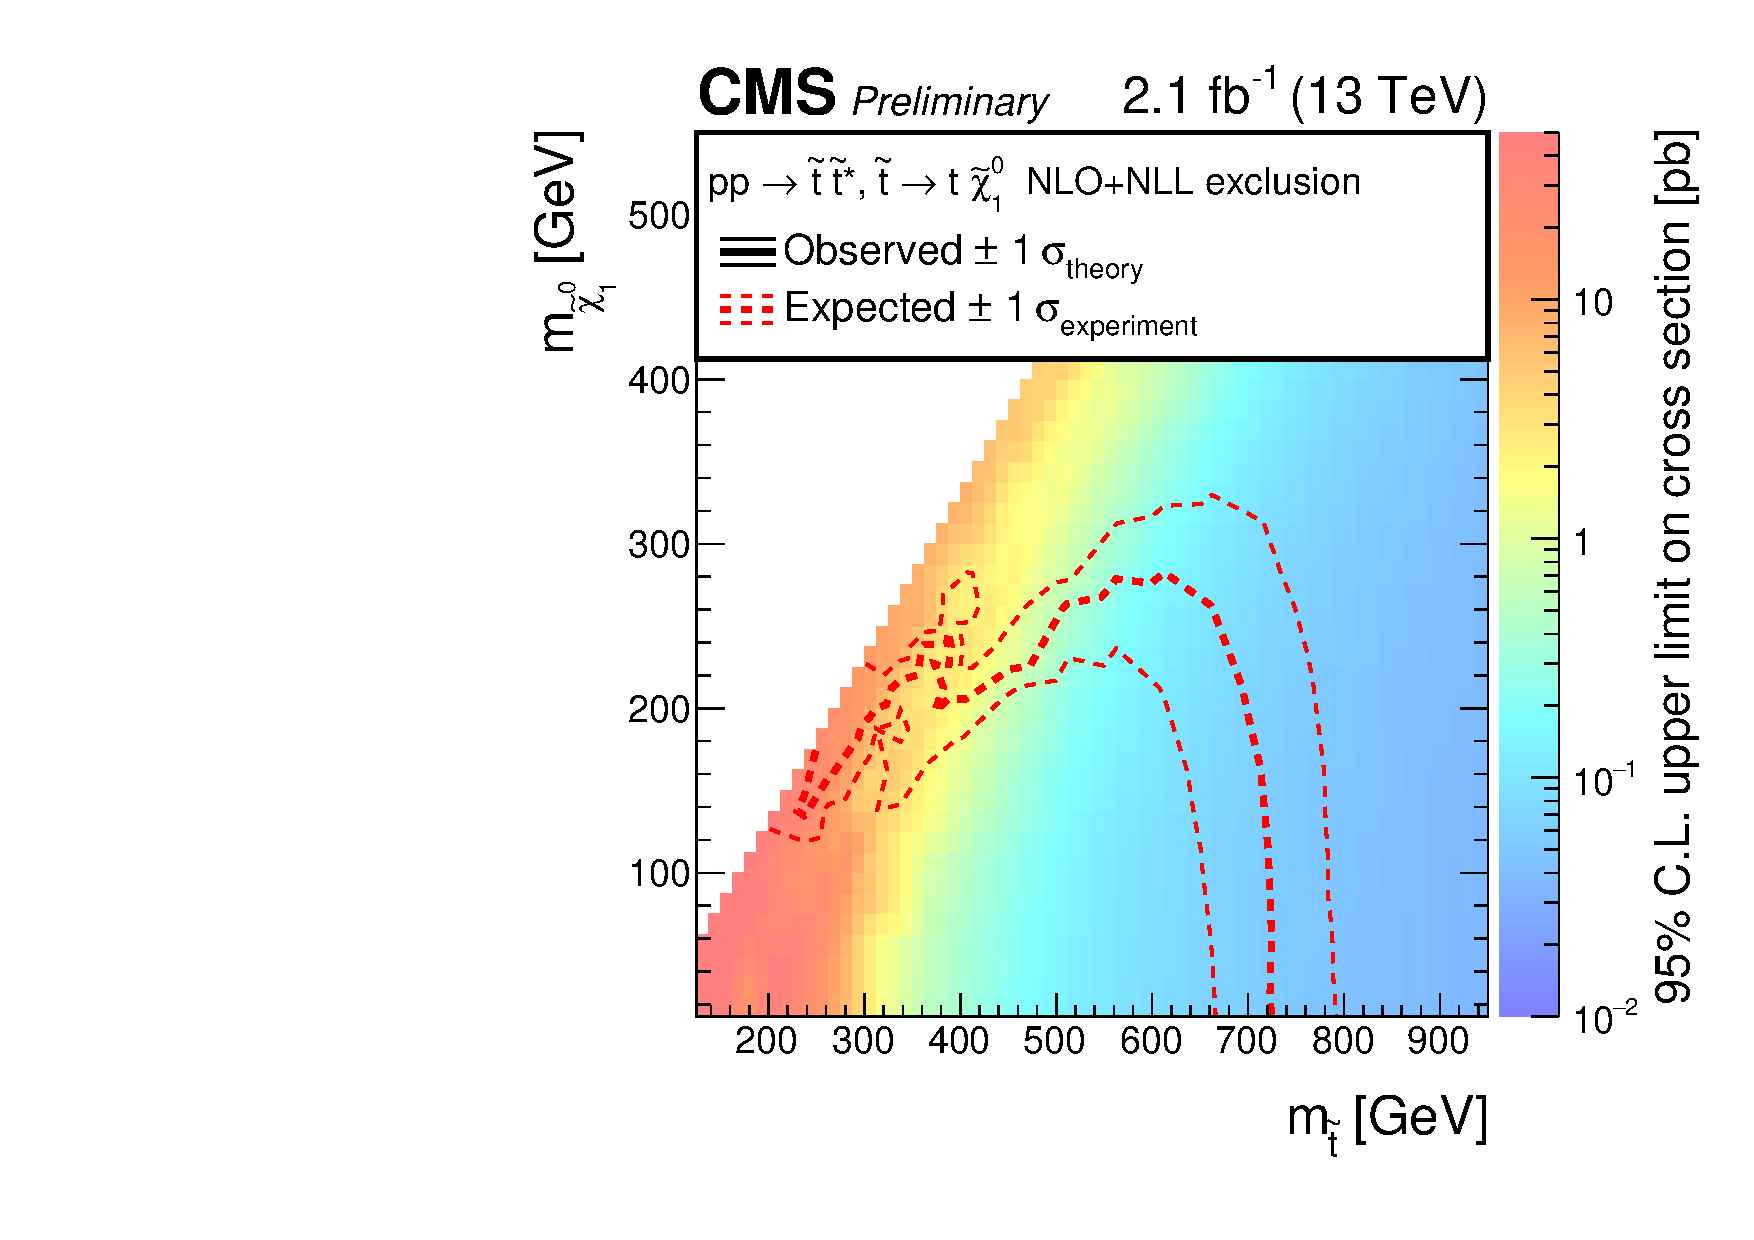
\includegraphics[width=0.8\textwidth]{plots_stop/T2ttstopXSEC.pdf}
\caption{\label{fig:limits:T2tt}Exclusion limit at 95\% CL for direct top-squark production with decay $\stone\to\PQt^{(*)}\PSGczDo$. \textcolor{red}{Once the final plot is here, we also need to add information about the different lines...} }
\end{figure}

\textcolor{red}{Section not finished yet.}

\section{Results}

A summary of the background expectations and the corresponding data counts for each signal
region is shown in Table \ref{tab:results} and shown in Fig/\ref{fig:results}.  The observed and predicted yields agree in all signal regions within about XX standard deviations. Therefore, we observe no evidence for top-squark pair production.

\begin{table}[htb]
\begin{center}
\caption{\label{tab:results} Results of the data- and simulation-driven background estimates together with the observed data yields for 2.3\fbinv collected during 2015 pp collisions. The uncertainties are the quadratic sums of statistical and systematic uncertainties.{\color{red} Data still blinded.}}
\begin{tabular}{|r|r@{\,$\pm$\,}lr@{\,$\pm$\,}lr@{\,$\pm$\,}lr@{\,$\pm$\,}l|r@{\,$\pm$\,}l|r|}
\hline
\multirow{2}{*}{\MET [GeV]} &  \multicolumn{2}{c|}{\multirow{2}{*}{Lost Lepton}} & \multicolumn{2}{c|}{$1\ell$ (not}  &  \multicolumn{2}{c|}{\multirow{2}{*}{$\ttbar\to1\ell$}} &  \multicolumn{2}{c|}{\multirow{2}{*}{$\cPZ\to\cPgn\cPagn$}} & \multicolumn{2}{c|}{Total} & \multirow{2}{*}{Data} \\
 & \multicolumn{2}{c|}{~} & \multicolumn{2}{c|}{from top)} & \multicolumn{2}{c|}{~} & \multicolumn{2}{c|}{~} & \multicolumn{2}{c|}{background} &  \\
\hline
 & \multicolumn{11}{l|}{Boosted High $\Delta M$}\\%: $3$ jets, $\MTtW>200\GeV$} \\
\hline
$>350$    & 0.84&0.23 & 0.98&0.62 & 0.05&0.05 & 0.28&0.08 & 2.15&0.67 & 0 \\
\hline
 & \multicolumn{11}{l|}{Low $\Delta M$}\\%: $\geq4$ jets, $\MTtW\leq200\GeV$} \\
\hline
$250-325$ & 19.27&2.76 & 0.55&0.55 & 0.76&0.76 & 0.63&0.12 & 21.21&2.92 & 0 \\
$>325$ & 7.64&1.28 & 0.38&0.38 & 0.34&0.34 & 0.27&0.08 & 8.63&1.38 & 0 \\
\hline
 & \multicolumn{11}{l|}{High $\Delta M$}\\%: $\geq4$ jets, $\MTtW>200\GeV$} \\
\hline
$250-350$ & 3.08&0.82 & 1.05&0.53 & 0.49&0.49 & 0.63&0.15 & 5.25&1.10 & 0 \\
$350-450$ & 0.83&0.23 & 0.82&0.49 & 0.12&0.12 & 0.38&0.10 & 2.15&0.56 & 0 \\
$>450$ & 0.59&0.21 & 0.95&0.67 & 0.07&0.07 & 0.34&0.15 & 1.95&0.72 & 0 \\
\hline
\end{tabular}
\end{center}
\end{table}

\begin{figure}[htb]
\centering
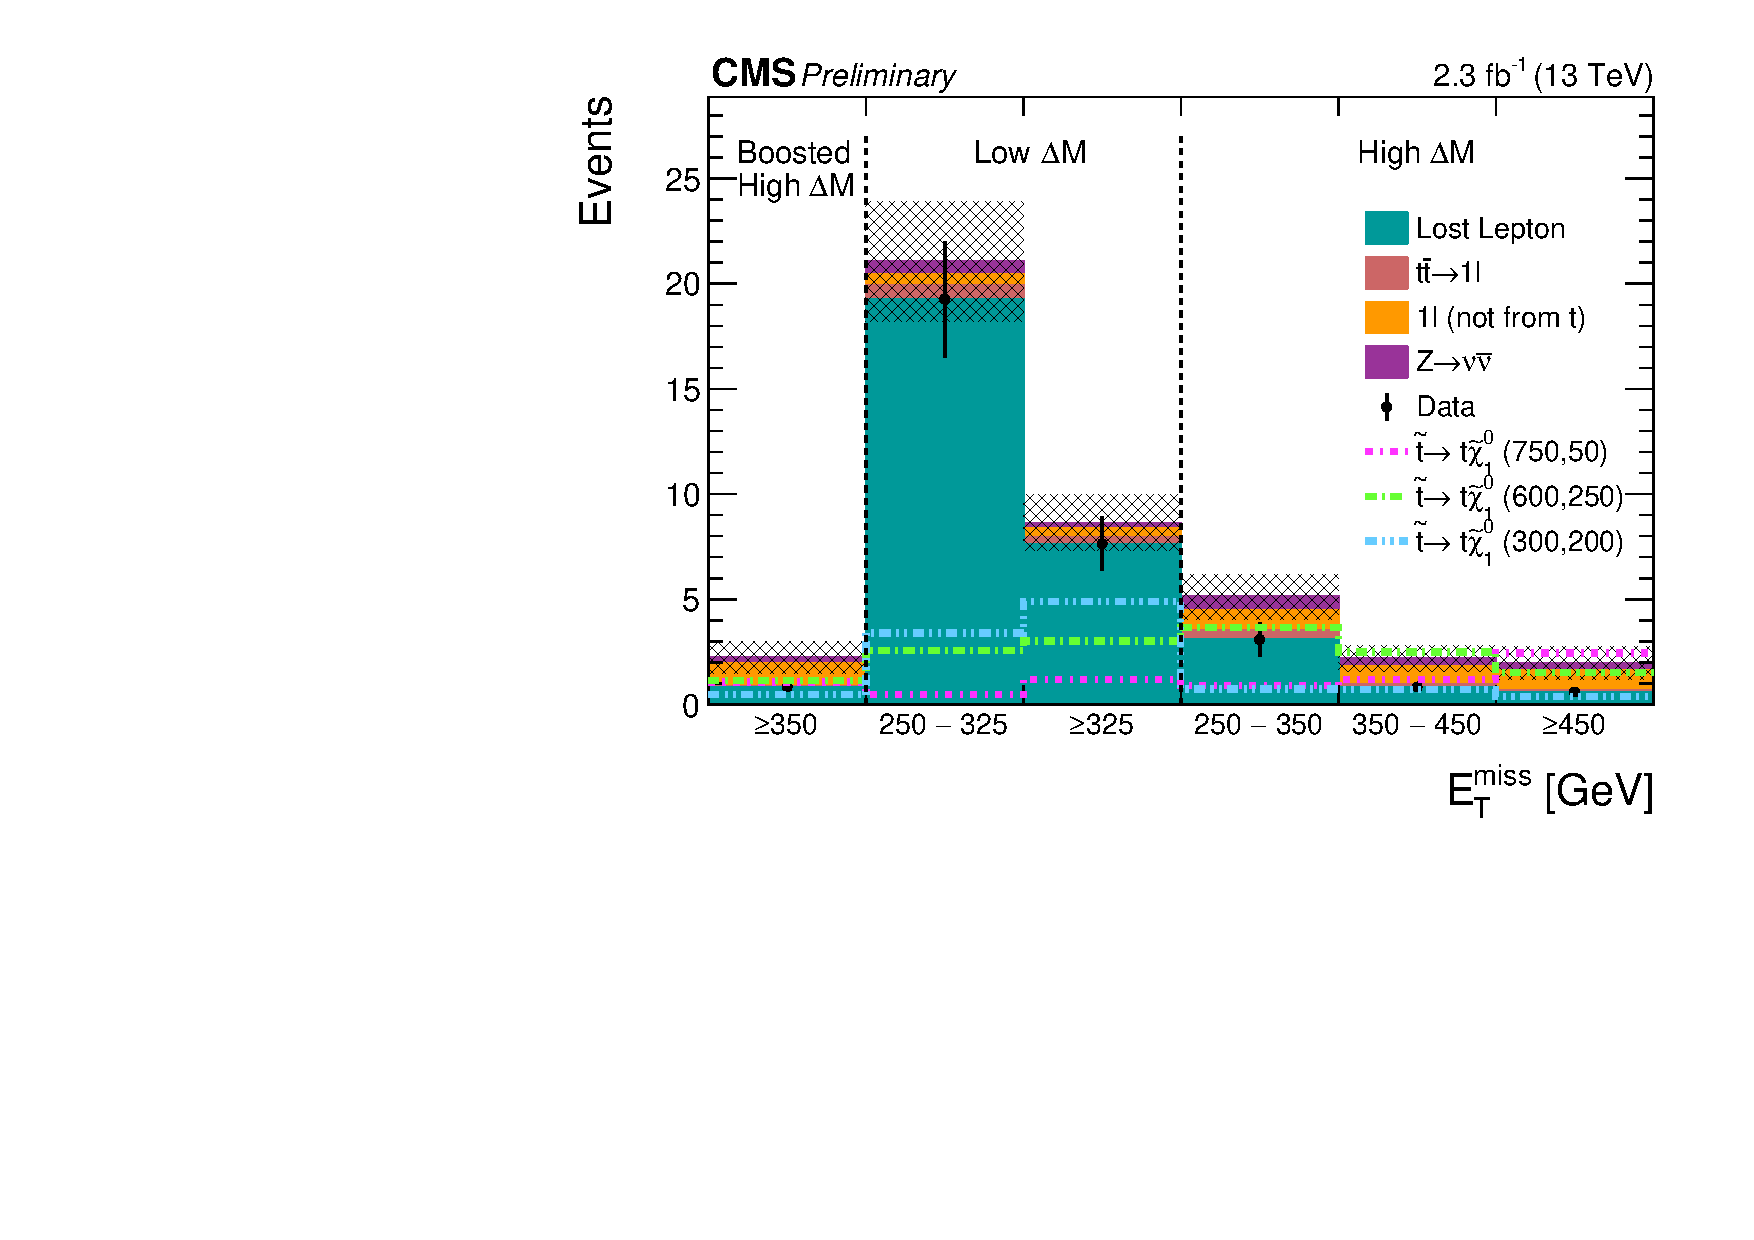
\includegraphics[width=0.90\textwidth]{plots_stop/Results_2p3fbinv.pdf}
\caption{\label{fig:results}Results of the data- and simulation-driven background estimates together with the observed data yields for 2.3\fbinv collected during 2015 pp collisions. The uncertainties, which are the quadratic sums of statistical and systematic uncertainties, are shown as shaded band. Three signal hypotheses are overlaid. {\color{red} Data still blinded, dots here are fake.}}
\end{figure}

The results of the search are interpreted in the context of models of top-squark pair production.  As discussed in Sec.\ref{sec:intro} we consider two different decay modes for the top-squark: directly to a top quark and a LSP or to a bottom quark and a chargino and then the chargino decays to the LSP.  We also consider the option where the chargino is almost mass-degenerate with the LSP.  In that case we can be sensitive to the mixed scenario, where one top decays to a top quark and a LSP and the other one to a bottom quark, a soft and undetected W boson and a LSP.  The systematic uncertainties are discussed in length in Sec.\ref{syst}.  We use all the search bins to calculate 95\% confidence level (CL) upper limits (UL) on the cross sections.  We calculate these upper limits using the LHC style CLS method\cite{Higgscombine}.

Figure~\ref{fig:limits:T2tt} shows the 95\% CL exclusion limits for $\Pp\Pp\to\stone\stone^*\to \PQt^{(*)}\PAQt^{(*)}\PSGczDo\PSGczDo$, together with the upper limit at 95\% CL on the excluded signal cross section.
\begin{figure}[htb]
\centering
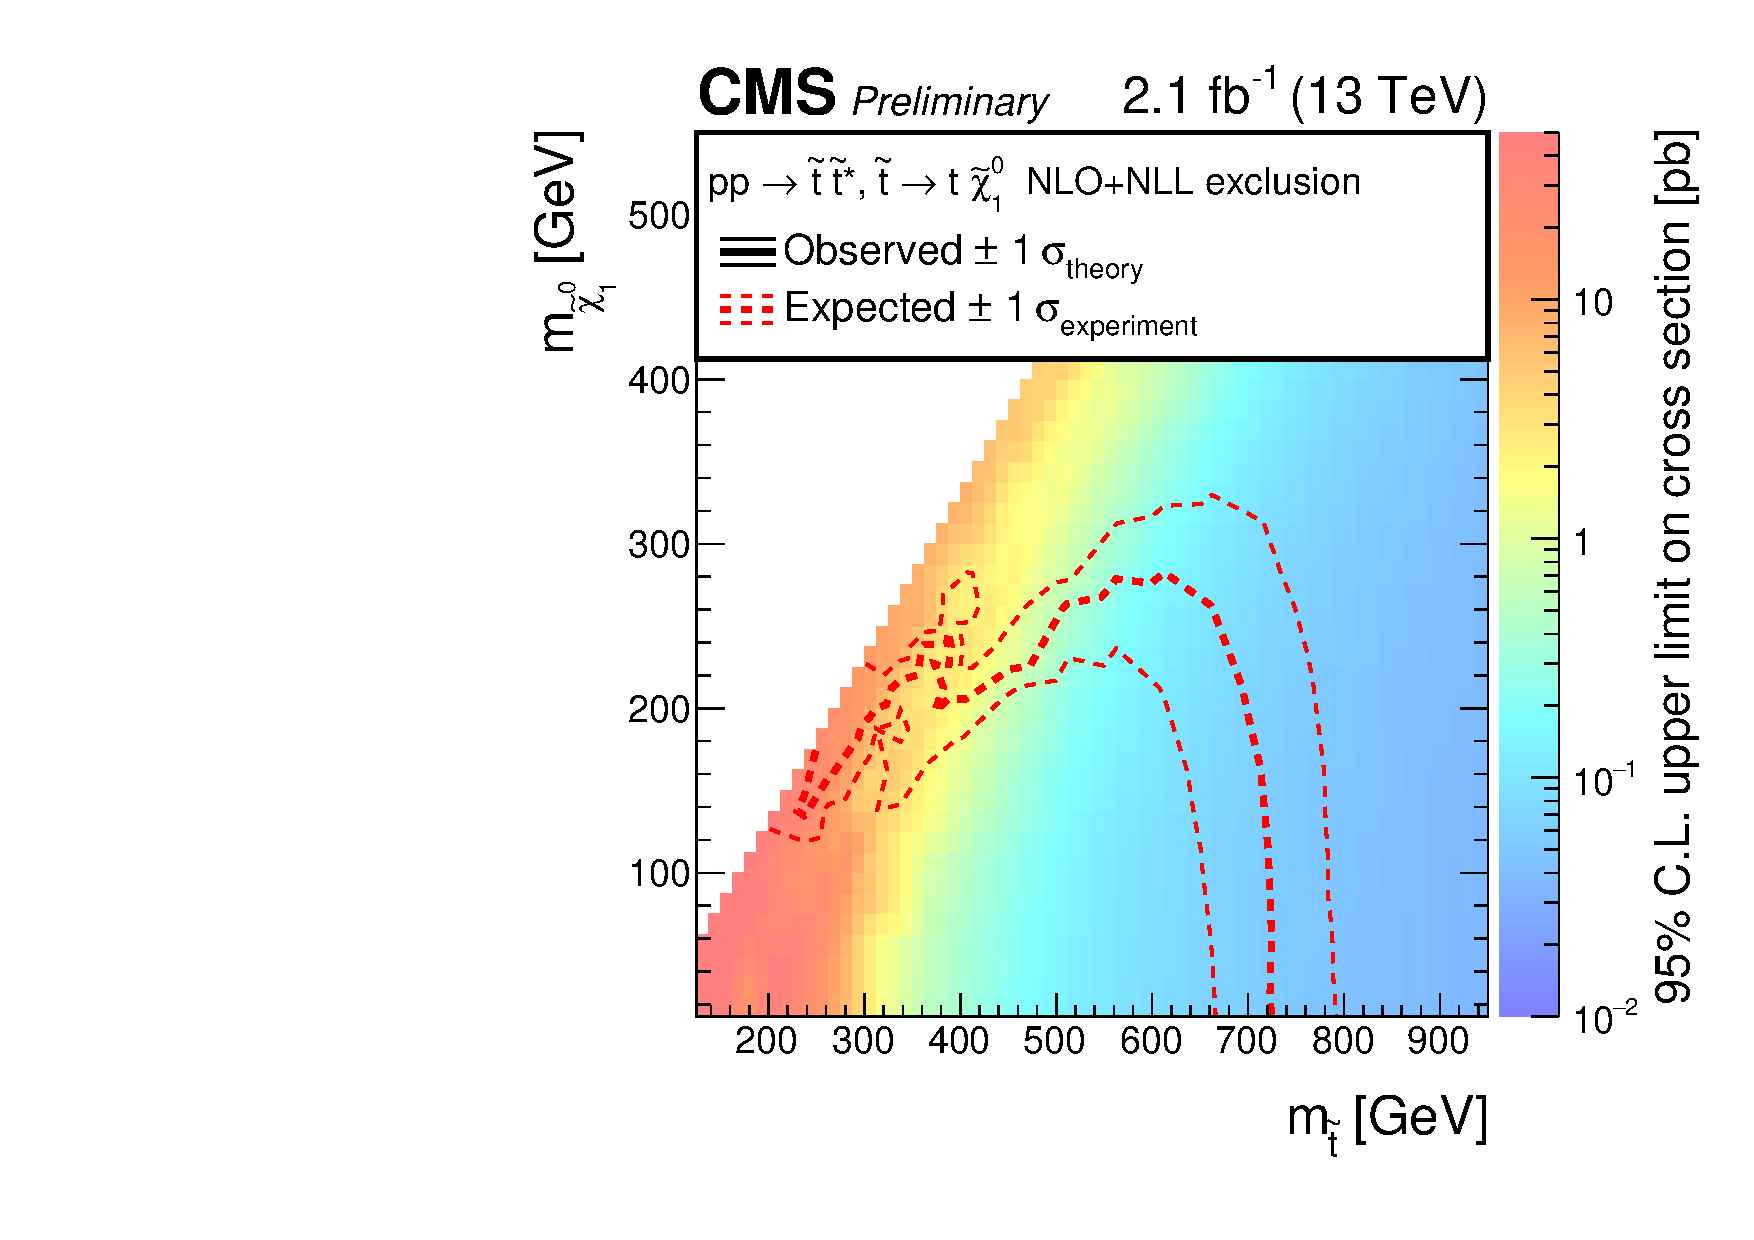
\includegraphics[width=0.8\textwidth]{plots_stop/T2ttstopXSEC.pdf}
\caption{\label{fig:limits:T2tt}Exclusion limit at 95\% CL for direct top-squark production with decay $\stone\to\PQt^{(*)}\PSGczDo$. \textcolor{red}{Once the final plot is here, we also need to add information about the different lines...} }
\end{figure}

\textcolor{red}{Section not finished yet.}

%\section{Summary}

\section{Summary}




% >> acknowledgments (for journal papers)
% Please include the latest version from https://twiki.cern.ch/twiki/bin/viewauth/CMS/Internal/PubAcknow.
%\begin{acknowledgments}...ack-text...\end{acknowledgments}
%

%% **DO NOT REMOVE BIBLIOGRAPHY**
\bibliography{auto_generated}   % will be created by the tdr script.

%% examples of appendices. **DO NOT PUT \end{document} at the end
%\clearpage
%\appendix

